% !TeX spellcheck = <none>
% Зачем: Определяет класс документа (То, как будет выглядеть документ)
% Примечание: параметр draft помечает строки, вышедшие за границы страницы, прямоугольником, в фильной версии его нужно удалить.
\documentclass[a4paper,14pt,russian,oneside,final]{extreport}

% Зачем: Установка кодировки исходных файлов.
\usepackage[utf8]{inputenc}

% Зачем: Делает результирующий PDF "searchable and copyable".
\usepackage{cmap}

% Зачем: Выбор внутренней TeX кодировки.
\usepackage[T2A]{fontenc}

% Зачем: Чтобы можно было использовать русские буквы в формулах, но в случае использования предупреждать об этом.
\usepackage[warn]{mathtext}

% Зачем: Учет особенностей различных языков.
\usepackage[russian]{babel}

% Зачем: Улучшает отображение русских шрифтов.
% Примечание: Требует шаманства при установке, инструкция http://plumbum-blog.blogspot.com/2010/06/miktex-28-pscyr-04d.html
%\usepackage{pscyr}


% Зачем: Добавляет поддержу дополнительных размеров текста 8pt, 9pt, 10pt, 11pt, 12pt, 14pt, 17pt, and 20pt.
% Почему: Пункт 2.1.1 Требований по оформлению пояснительной записки.
\usepackage{extsizes}


% Зачем: Длинна, пимерно соответвующая 5 символам
% Почему: Требования содержат странное требование про отсупы в 5 символов (для немоноширинного шрифта :| )
\newlength{\fivecharsapprox}
\setlength{\fivecharsapprox}{6ex}


% Зачем: Добавляет отступы для абзацев.
% Почему: Пункт 2.1.3 Требований по оформлению пояснительной записки.
\usepackage{indentfirst}
\setlength{\parindent}{\fivecharsapprox} % Примерно соответсвует 5 символам.


% Зачем: Настраивает отступы от границ страницы.
% Почему: Пункт 2.1.2 Требований по оформлению пояснительной записки.
\usepackage[left=3cm,top=2.0cm,right=1cm,bottom=2.0cm]{geometry}


% Зачем: Настраивает межстрочный интервал, для размещения 40 +/- 3 строки текста на странице.
% Почему: Пункт 2.1.1 Требований по оформлению пояснительной записки.
\usepackage[nodisplayskipstretch]{setspace} 
\setstretch{1.1}
%\onehalfspacing

% Зачем: Выбор шрифта по-умолчанию. 
% Почему: Пункт 2.1.1 Требований по оформлению пояснительной записки.
% Примечание: В требованиях не указан, какой именно шрифт использовать. По традиции используем TNR.
\renewcommand{\rmdefault}{ftm} % Times New Roman


% Зачем: Отключает использование изменяемых межсловных пробелов.
% Почему: Так не принято делать в текстах на русском языке.
\frenchspacing


% Зачем: Сброс счетчика сносок для каждой страницы
% Примечание: в "Требованиях по оформлению пояснительной записки" не указано, как нужно делать, но в других БГУИРовских докуметах рекомендуется нумерация отдельная для каждой страницы
\usepackage{perpage}
\MakePerPage{footnote}


% Зачем: Добавляет скобку 1) к номеру сноски
% Почему: Пункты 2.9.2 и 2.9.1 Требований по оформлению пояснительной записки.
\makeatletter 
\def\@makefnmark{\hbox{\@textsuperscript{\normalfont\@thefnmark)}}}
\makeatother


% Зачем: Расположение сносок внизу страницы
% Почему: Пункт 2.9.2 Требований по оформлению пояснительной записки.
\usepackage[bottom]{footmisc}


% Зачем: Переопределяем стандартную нумерацию, т.к. в отчете будут только section и т.д. в терминологии TeX
\makeatletter
\renewcommand{\thesection}{Раздел \arabic{section} }
\renewcommand{\thesubsection}{\arabic{section}.\arabic{subsection}}
\makeatother


% Зачем: Пункты (в терминологии требований) в терминологии TeX subsubsection должны нумероваться
% Почему: Пункт 2.2.3 Требований по оформлению пояснительной записки.
\setcounter{secnumdepth}{3}


% Зачем: Настраивает отступ между таблицей с содержанимем и словом СОДЕРЖАНИЕ
% Почему: Пункт 2.2.7 Требований по оформлению пояснительной записки.
\usepackage{tocloft}
\setlength{\cftbeforetoctitleskip}{-1em}
\setlength{\cftaftertoctitleskip}{1em}

\usepackage{fancyhdr}
\pagestyle{fancy}
\fancyhf{}
\fancyhead[R]{\thepage}
\fancyheadoffset{0mm}
\fancyfootoffset{0mm}
\setlength{\headheight}{17pt}
\renewcommand{\headrulewidth}{0pt}
\renewcommand{\footrulewidth}{0pt}
\fancypagestyle{plain}{ 
    \fancyhf{}
    \rhead{\thepage}}

% Зачем: Определяет отступы слева для записей в таблице содержания.
% Почему: Пункт 2.2.7 Требований по оформлению пояснительной записки.
\makeatletter
\renewcommand{\l@section}{\@dottedtocline{1}{0.5em}{4.5em}}
\renewcommand{\l@subsection}{\@dottedtocline{2}{2.0em}{2.2em}}

\makeatother

% Зачем: Задает стиль заголовков раздела жирным шрифтом, прописными буквами, без точки в конце
% Почему: Пункты 2.1.1, 2.2.5, 2.2.6 и ПРИЛОЖЕНИЕ Л Требований по оформлению пояснительной записки.
\makeatletter
\renewcommand\section{%
  \clearpage\@startsection {section}{1}%
   	{\z@}%
    {-1em \@plus -1ex \@minus -.2ex}%
    {1em \@plus .2ex}%
    {\raggedright\hyphenpenalty=10000\normalfont\large\bfseries\MakeUppercase}}
\makeatother


% Зачем: Задает стиль заголовков подразделов
% Почему: Пункты 2.1.1, 2.2.5 и ПРИЛОЖЕНИЕ Л Требований по оформлению пояснительной записки.
\makeatletter
\renewcommand\subsection{%
  \@startsection{subsection}{2}%
   	{\z@}%
   	  {-1em \@plus -1ex \@minus -.2ex}%
    {1em \@plus .2ex}%
    {\raggedright\hyphenpenalty=10000\normalfont\normalsize\bfseries}}
\makeatother


% Зачем: Задает стиль заголовков пунктов
% Почему: Пункты 2.1.1, 2.2.5 и ПРИЛОЖЕНИЕ Л Требований по оформлению пояснительной записки.
\makeatletter
\renewcommand\subsubsection{
  \@startsection{subsubsection}{3}%
    {\fivecharsapprox}%
    {-1em \@plus -1ex \@minus -.2ex}%
    {\z@}%
    {\raggedright\hyphenpenalty=10000\normalfont\normalsize\bfseries}}
\makeatother

% Зачем: для оформления введения и заключения, они должны быть выровнены по центру.
% Почему: Пункты 1.1.15 и 1.1.11 Требований по оформлению пояснительной записки.
\makeatletter
\newcommand\sectioncentered{%
  \clearpage\@startsection {section}{1}%
    {\z@}%
    {-1em \@plus -1ex \@minus -.2ex}%
    {1em \@plus .2ex}%
    {\raggedright\hyphenpenalty=10000\normalfont\large\bfseries\MakeUppercase}%
    }
\makeatother



% Зачем: Задает стиль библиографии
% Почему: Пункт 2.8.6 Требований по оформлению пояснительной записки.
\bibliographystyle{styles/belarus-specific-utf8gost780u}


% Зачем: Пакет для вставки картинок
% Примечание: Объяснение, зачем final - http://tex.stackexchange.com/questions/11004/why-does-the-image-not-appear
\usepackage[final]{graphicx}
\DeclareGraphicsExtensions{.pdf,.png,.jpg,.eps}


% Зачем: Директория в которой будет происходить поиск картинок
\graphicspath{{figures/}}


% Зачем: Добавление подписей к рисункам
\usepackage[nooneline]{caption}
\usepackage{subcaption}

% Зачем: Задание подписей, разделителя и нумерации частей рисунков
% Почему: Пункт 2.5.5 Требований по оформлению пояснительной записки.
\DeclareCaptionLabelFormat{stbfigure}{Рис #2}
\DeclareCaptionLabelFormat{stbtable}{Таблица #2}
\DeclareCaptionLabelSeparator{stb}{~--~}
\captionsetup{labelsep=stb}
\captionsetup[figure]{labelformat=stbfigure,justification=centering}
\captionsetup[table]{labelformat=stbtable,justification=raggedleft}
\renewcommand{\thesubfigure}{\asbuk{subfigure}}

% Зачем: Окружения для оформления формул
% Почему: Пункт 2.4.7 требований по оформлению пояснительной записки и специфические требования различных кафедр
\usepackage{tabularx}

\newenvironment{explanation}
    {
    %%% Следующие строки определяют специфические требования кафедр. Раскоменнтируйте нужные 2 строки
    %% стандартный абзац, Кафедра информатики
    \par 
    \tabularx{\textwidth-\fivecharsapprox}{@{}ll@{ --- } X }
    %% без отступа, Кафедра экономической информатики
    %\noindent 
    %\tabularx{\textwidth}{@{}ll@{ --- } X }
    }
    { 
    \\[\parsep]
    \endtabularx
    }


% Зачем: Удобная вёрстка многострочных формул, масштабирующийся текст в формулах, формулы в рамках и др
\usepackage{amsmath}


% Зачем: Поддержка ажурного и готического шрифтов 
\usepackage{amsfonts}


% Зачем: amsfonts + несколько сотен дополнительных математических символов
\usepackage{amssymb}


% Зачем: Окружения «теорема», «лемма»
\usepackage{amsthm}
\newtheorem{definition}{Определение}
\newtheorem{theorem}{Теорема}


% Зачем: Производить арифметические операции во время компиляции TeX файла
\usepackage{calc}

% Зачем: Производить арифметические операции во время компиляции TeX файла
\usepackage{fp}

% Зачем: Пакет для работы с перечислениями
\usepackage{enumitem}
\makeatletter
 \AddEnumerateCounter{\asbuk}{\@asbuk}{щ)}
\makeatother


% Зачем: Устанавливает символ начала простого перечисления
% Почему: Пункт 2.3.5 Требований по оформлению пояснительной записки.
\setlist{nolistsep}


% Зачем: Устанавливает символ начала именованного перечисления
% Почему: Пункт 2.3.8 Требований по оформлению пояснительной записки.
\renewcommand{\labelenumi}{\asbuk{enumi})}
\renewcommand{\labelenumii}{\arabic{enumii})}

% Зачем: Устанавливает отступ от границы документа до символа списка, чтобы этот отступ равнялся отступу параграфа
% Почему: Пункт 2.3.5 Требований по оформлению пояснительной записки.

\setlist[itemize,0]{itemindent=\parindent + 2.2ex,leftmargin=0ex,label=--}
\setlist[enumerate,1]{itemindent=\parindent + 2.7ex,leftmargin=0ex}
\setlist[enumerate,2]{itemindent=\parindent + \parindent - 2.7ex}

% Зачем: Включение номера раздела в номер формулы. Нумерация формул внутри раздела.
\newcounter{forsec}
\setcounter{forsec}{1}

\AtBeginDocument{\numberwithin{equation}{forsec}}

% Зачем: Включение номера раздела в номер таблицы. Нумерация таблиц внутри раздела.
\AtBeginDocument{\numberwithin{table}{forsec}}

% Зачем: Включение номера раздела в номер рисунка. Нумерация рисунков внутри раздела.
\AtBeginDocument{\numberwithin{figure}{forsec}}


% Зачем: Дополнительные возможности в форматировании таблиц
\usepackage{makecell}
\usepackage{multirow}
\usepackage{array}


% Зачем: "Умная" запятая в математических формулах. В дробных числах не добавляет пробел
% Почему: В требованиях не нашел, но в русском языке для дробных чисел используется {,} а не {.}
\usepackage{icomma}

% Зачем: макрос для печати римских чисел
\makeatletter
\newcommand{\rmnum}[1]{\romannumeral #1}
\newcommand{\Rmnum}[1]{\expandafter\@slowromancap\romannumeral #1@}
\makeatother


% Зачем: Управление выводом чисел.
\usepackage{sistyle}
\SIdecimalsign{,}

% Зачем: inline-коментирование содержимого.
\newcommand{\ignore}[2]{\hspace{0in}#2}


% Зачем: Возможность коментировать большие участки документа
\usepackage{verbatim}


\usepackage{xcolor}


% Зачем: Оформление листингов кода
% Примечание: final нужен для переопределения режима draft, в котором листинги не выводятся в документ.
\usepackage[final]{listings}


% Зачем: настройка оформления листинга для языка F#
\definecolor{bluekeywords}{rgb}{0.13,0.13,1}
\definecolor{greencomments}{rgb}{0,0.5,0}
\definecolor{turqusnumbers}{rgb}{0.17,0.57,0.69}
\definecolor{redstrings}{rgb}{0.5,0,0}

\renewcommand{\lstlistingname}{Листинг}

\lstdefinelanguage{FSharp}
    {morekeywords={abstract,and,as,assert,base,begin,class,default,delegate,do,done,downcast,downto,elif,else,end,exception,extern,false,finally,for,fun,function,global,if,in,inherit,inline,interface,internal,lazy,let,let!,match,member,module,mutable,namespace,new,not,null,of,open,or,override,private,rec,return,return!,select,static,struct,then,to,true,try,type,upcast,use,use!,val,void,when,while,with,yield,yield!,asr,land,lor,lsl,lsr,lxor,mod,sig,atomic,break,checked,component,const,constraint,constructor,continue,eager,event,external,fixed,functor,include,method,mixin,object,parallel,process,protected,pure,sealed,tailcall,trait,virtual,volatile, def, import, from, Class},
    keywordstyle=\bfseries\color{bluekeywords},
    sensitive=false,
    morecomment=[l][\color{greencomments}]{///},
    morecomment=[l][\color{greencomments}]{//},
    morecomment=[s][\color{greencomments}]{{(*}{*)}},
    morestring=[b]",
    stringstyle=\color{redstrings},
    }

\lstdefinestyle{fsharpstyle}{
   xleftmargin=0ex,
   language=FSharp,
   basicstyle=\footnotesize\ttfamily,
   breaklines=true,
   columns=fullflexible
}

\lstdefinestyle{csharpinlinestyle} {
  language=[Sharp]C,
  morekeywords={yield,var,get,set,from,select,partial,where,async,await},
  breaklines=true,
  columns=fullflexible,
  basicstyle=\footnotesize\ttfamily
}

\lstdefinestyle{csharpstyle}{
  language=[Sharp]C,
  frame=lr,
  rulecolor=\color{blue!80!black}}


% Зачем: Нумерация листингов в пределах секции
\AtBeginDocument{\numberwithin{lstlisting}{section}}

\usepackage[normalem]{ulem}

\usepackage[final,hidelinks]{hyperref}
% Моноширинный шрифт выглядит визуально больше, чем пропорциональный шрифт, если их размеры одинаковы. Искусственно уменьшаем размер ссылок.
\renewcommand{\UrlFont}{\small\rmfamily\tt}

\usepackage[square,numbers,sort&compress]{natbib}
\setlength{\bibsep}{0em}

% Магия для подсчета разнообразных объектов в документе
\usepackage{lastpage}
\usepackage{totcount}
\regtotcounter{section}

\usepackage{etoolbox}

\newcounter{totfigures}
\newcounter{tottables}
\newcounter{totreferences}
\newcounter{totequation}

\providecommand\totfig{} 
\providecommand\tottab{}
\providecommand\totref{}
\providecommand\toteq{}

\makeatletter
\AtEndDocument{%
  \addtocounter{totfigures}{\value{figure}}%
  \addtocounter{tottables}{\value{table}}%
  \addtocounter{totequation}{\value{equation}}
  \immediate\write\@mainaux{%
    \string\gdef\string\totfig{\number\value{totfigures}}%
    \string\gdef\string\tottab{\number\value{tottables}}%
    \string\gdef\string\totref{\number\value{totreferences}}%
    \string\gdef\string\toteq{\number\value{totequation}}%
  }%
}
\makeatother

\pretocmd{\section}{\addtocounter{totfigures}{\value{figure}}\setcounter{figure}{0}}{}{}
\pretocmd{\section}{\addtocounter{tottables}{\value{table}}\setcounter{table}{0}}{}{}
\pretocmd{\section}{\addtocounter{totequation}{\value{equation}}\setcounter{equation}{0}}{}{}
\pretocmd{\bibitem}{\addtocounter{totreferences}{1}}{}{}



% Для оформления таблиц не влязящих на 1 страницу
\usepackage{longtable}

% Для включения pdf документов в результирующий файл
\usepackage{pdfpages}


\usepackage{wrapfig}

\usepackage{multirow}

\renewcommand{\rmdefault}{cmr} % Шрифт с засечками
\renewcommand{\sfdefault}{cmss} % Шрифт без засечек
\renewcommand{\ttdefault}{cmtt} % Моноширинный шрифт
% Зачем: Переносы в словах с тире.
% Тире в словае заменяем на \hyph: аппаратно\hyphпрограммный.
% https://stackoverflow.com/questions/2193307/how-to-get-latex-to-hyphenate-a-word-that-contains-a-dash#
\def\hyph{-\penalty0\hskip0pt\relax}



\newcommand{\csharp}{C\#}
\newcommand{\fsharp}{F\#}
\newcommand{\vbnet}{Visual Basic~.NET}
\newcommand{\cpp}{C\texttt{\hspace{-0.3ex}+\hspace{-0.25ex}+}}
\newcommand{\cppcli}{Visual \cpp{}/CLI}
\newcommand{\dotnet}{Microsoft .NET}
\newcommand{\netfx}{.NET Framework}
\newcommand{\java}{Java}
\newcommand{\python}{Python}

\begin{document}

%\begin{titlepage}
  \begin{center}
   Министерство Образования Украины\\[1em]
    Учреждение образования\\
   Одеський національний університет імені І. І. Мечникова\\[1em]

    \begin{minipage}{\textwidth}
      \begin{flushleft}
        \begin{tabular}{ l l }
          Институт & Інститут математики, економіки та механіки\\
         Факультет   & Прикладная математика
        \end{tabular}
      \end{flushleft}
    \end{minipage}\\[1em]

   

   



    
   
    
    \vfill
    {\normalsize Одесса 2016}
  \end{center}
\end{titlepage}
 % page 1

%\input{abstract} % page 2

%\input{diploma_task} % pages 3 and 4. printed separately

%\input{annotation} % not part of report

%\input{feedback} % not part of report

%\input{review} % not part of report
\includepdf{title}

\setcounter{page}{2}

% Зачем: Содержание пишется полужирным шрифтом, по центру всеми заглавными буквами
% Почему: Пункт 2.2.7 Требований по оформлению пояснительной записки.
\renewcommand \contentsname {\centerline{\bfseries\large{\MakeUppercase{зміст}}}}

% Зачем: Не захламлять основной файл
% Примечание: \small\selectfont злостный хак, чтобы уменьшить размер шрифта в ToC 
{

\normalsize\selectfont
\tableofcontents
\newpage
}

%	\begin{equation}
	r^g> \bar{r^g}(R) = \left\{ 
	\begin{aligned} 
	&0=0, &&\text{если } R=0
	\\
	&0=0, &&\text{если } 	R\in(0; \frac{1}{2})
	\\
	&0=0&&\text{если } 	R\in( \frac{1}{2};1)
	\end{aligned}
	\right.		
	\end{equation}


\sectioncentered*{Вступ}
\addcontentsline{toc}{section}{Вступ}

Актуальність макроекономічних моделей, розглянутих у роботі, обумовлена
тим, що вони являють собою спробу об'єднати два математичних підходу до
моделювання реальних процесів управління і прийняття рішень. 

Перший --- теоретико-ігровий --- підхід дозволяє розглядати ситуації
конфлікту інтересів. Навіть сутєво спрощені моделі у вигляді біматричних ігор
є основою для цікавих висновків прикладного характеру.

Другий підхід полягає в розгляді конфлікту як явища протяжного у
часi, динамічного процесу прийняття рішень протиборчими сторонами.
Разом з класичними повторюваними іграми останнім часом активно
вивчаються гри на тимчасових шкалах, тобто iгри, в яких час для одного або
всіх гравців влаштовано складніше, ніж просто множина $\mathbb{N}_0$.

У даній дипломній роботі, відштовхуючись від відомих результатів по вивченню
моделі Барро --- Гордона на тимчасових шкалах, запропонована і дослiджена модель
взаємодії профспілки і фірми - монополіста.  Розроблене програмне
забезпечення дозволило шляхом імітаційного моделювання дослiдити властивості
запропонованої моделі та сформулювати певні висновки про способи
формування довгострокової рівноваги.

Структура роботи наступна: в розділі 1 коротко викладаються елементи теорії ігор і
аналізу на тимчасових шкалах. У розділі 2 розглядається теоретичний базис
обох розглянутих моделей. У розділі 3 викладаються результати комп'ютерних
експериментів з вивченими моделями, далі формулюються висновки. Завершує
текст роботи список використаної літератури і додаток, в якому наведен
прокоментований код програми.


\section{Основные понятия и определения}
\subsection{Элементы теории игр}

\begin{definition}
	$(S,H)$ --- не кооперативная игра $n$ лиц в нормальной
	форме, где $S$ --- набор чистых стратегий, а $H$ --- набор выигрышей. Когда
	каждый игрок $i \in \left\{1,\dots,n\right\}$  выбирает стратегию $x_i
	\in S$  в профиле стратегий $x=(x_1,\dots,x_n)$, игрок $i$  получает
	выигрыш $H_i(x)$. Профиль стратегий $x^* \in S$   является равновесием
	по Нэшу, если изменение своей стратегии с $x_i^*$  на $x_i$  не выгодно
	ни одному игроку $i$, то есть $\forall i : H_i(x^*) \geqslant H_i(x_i,
	x_{-i}^*)$.
\end{definition}
	
\begin{definition}
	Равновесие по Нэшу называется безупречным по под-играм, если и только если оно
	является равновесием по Нэшу для каждой под-игры. 
\end{definition}

\begin{definition}
Парето-оптимальность в смысле теории игр характеризует такую ситуацию, при которой невозможно улучшить исход игры для одного игрока без его ухудшения для других игроков.
\end{definition}

\begin{definition}
	Инфляция --- повышение общего уровня цен на товары и услуги.
\end{definition}

\begin{definition}
	Индексация заработной платы --- повышение заработных плат с целью частичной защиты населения от роста потребительских цен на товары и услуги.
\end{definition}

\begin{definition}
	Любое совершенное равновесие по под-играм (SPNE), в котором оба игрока выбирают стратегию L во всех своих ходах, назовём \textbf{совершенным равновесием Рамсея по под-играм (Ramsey SPNE)}~\cite{libich2008macroeconomic}
\end{definition}

\subsection{Элементы анализа на временных шкалах}

Сведения из теории временных шкал приводятся следуя двум основным
источникам \cite{Bohner,BohnerAdv}.

\begin{definition}
	Под временной шкалой понимается непустое замкнутое подмножество множества
	вещественных чисел, она обозначается символом $\mathbb{T}$.
	Свойства временной шкалы определяются тремя функциями:
	\begin{itemize}
		\item[1)] оператор перехода вперед:
		\[
		\sigma(t) = \inf\left\{s \in \mathbb{T}: s > t\right\};
		\]
		\item[2)] оператор перехода назад:
		\[
		\rho(t) = \sup\left\{s \in \mathbb{T}: s < t\right\},
		\]
		(при этом полагается $\inf\varnothing = \sup{\mathbb{T}}$ и $\sup\varnothing = \inf{\mathbb{T}}$);
		\item[3)] функция зернистости
		$$\mu(t) = \sigma(t) - t.$$
	\end{itemize}
\end{definition}
Поведение операторов перехода вперед и назад в конкретной точке временной шкалы
определяет тип этой точки. Соответствующая классификация точек представлена в
таблице~(\ref{tab:pointclass}).
\begin{table}[h]

	\centering		
		\caption{}	
		 Классификация точек временной шкалы\\
		\begin{tabular}{|l|l|}
			\hline
			$t$ справа рассеянная & $t < \sigma(t)$ \\
			$t$ справа плотная    & $t = \sigma(t)$ \\
			$t$ слева рассеянная  & $ \rho(t) < t $ \\
			$t$ слева плотная     & $ \rho(t) = t $ \\
			$t$ изолированная      & $\rho(t) < t < \sigma(t)$ \\
			$t$ плотная           & $\rho(t) = t = \sigma(t)$ \\
			\hline
		\end{tabular}
	
	\label{tab:pointclass}
\end{table}

\begin{definition}
	 Множество $\mathbb{T}^\kappa$ определим как:
	 \[
	 \mathbb{T}^\kappa =
	 \begin{cases}
	 \mathbb{T}\setminus \left\{M\right\}, & \text{ если }
	 \exists \text{ справа рассеянная точка } M \in \mathbb{T}:\\
	 & M = \sup\mathbb{T}, \sup\mathbb{T}<\infty  \\
	 \mathbb{T} , & \text{ в противном случае}.
	 \end{cases}
	 \]
	 Далее полагаем $\left[a, b\right] =
	 \left\{t \in \mathbb{T} : a \leqslant t \leqslant b\right\}$.
\end{definition}

\begin{definition}
    Пусть $f:\mathbb{T} \rightarrow \mathbb{R}$ и $t \in \mathbb{T}^\kappa$.
    Число $f^{\Delta}(t)$ называется $\Delta$-производной функции $f$ в точке $t$,
    если $\forall \varepsilon > 0$ найдется такая окрестность
    $U$ точки $t$ (то есть, $U = (t - \delta, t + \delta) \cap \mathbb{T}, \delta < 0$),
    что
    \[
    \left|f(\sigma(t)) - f(s) - f^{\Delta}(t)(\sigma(t)-s)\right| \leqslant
        \varepsilon\left|\sigma(t) - s\right| \quad \forall s \in U.
    \]
\end{definition}

\begin{definition}
    Если $f^{\Delta}(t)$ существует $\forall t \in \mathbb{T}^\kappa$,
    то $f:\mathbb{T} \rightarrow \mathbb{R}$ называется $\Delta$-дифферен\-ци\-ру\-емой
    на $\mathbb{T}^\kappa$. Функция $f^{\Delta}(t): \mathbb{T}^\kappa \rightarrow \mathbb{R}$
    называется дельта-производной функции $f$ на $\mathbb{T}^\kappa$.
\end{definition}

Если $f$ дифференцируемая в $t$, то
\[
    f(\sigma(t)) = f(t) + \mu(t)f^{\Delta}(t).
\]

\begin{definition}
    Функция $f:\mathbb{T} \rightarrow \mathbb{R}$ называется регулярной,
    если во всех плотных справа точках временной шкалы $\mathbb{T}$ она имеет
    конечные правосторонние пределы, а во всех слева плотных точках она имеет
    конечные левосторонние пределы.
\end{definition}

\begin{definition}
    Функция $f:\mathbb{T} \rightarrow \mathbb{R}$ называется $rd$-непрерывной,
    если в справа плотных точках она непрерывна, а в слева плотных точках имеет
    конечные левосторонние пределы. Множество таких функций обозначается
    $C_{rd} = C_{rd}(\mathbb{T})$, а множество дифференцируемых функций,
    производная которых $rd$-непрерывна, обозначается как
    $C_{rd}^1 = C_{rd}^1(\mathbb{T})$.
\end{definition}


\begin{definition}
Для любой регулярной функции $f(t)$ существует функция $F$,
дифференцируемая в области $D$ такая, что для всех $t \in D$
выполняется равенство $$F^{\Delta}(t) = f(t).$$
Эта функция называется пред-первообразной для $f(t)$ и
определяется она неоднозначно.
\end{definition}

Неопределенный интеграл на временной шкале имеет вид:
\[
    \int{f(t) \Delta t} = F(t) + C,
\]
где $C$ --- произвольная константа интегрирования, а $F(t)$ --- пред-перво\-образ\-ная для $f(t)$.
Далее, если для всех $t \in \mathbb{T}^\kappa$ выполняется $F^{\Delta}(t) =
f(t)$, где $f:\mathbb{T}\rightarrow\mathbb{R}$ --- $rd$-непрерывная функция, то
$F(t)$ называется первообразной функции $f(t)$. Если $t_0 \in \mathbb{T}$, то
$\displaystyle F(t) = \int\limits_{t_0}^t{f(s) \Delta s}$ для всех $t$.
Определенный $\Delta$-интеграл для любых $r,s \in \mathbb{T}$ определяется как
\[
    \int\limits_r^s{f(t)\Delta t} = F(s) - F(r).
\]


\setcounter{forsec}{2}
\section{Макроекономічні моделі на часових шкалах}
\subsection{Класична модель Барро-Гордона}
\label{sec:domain}

\paragraph{} Класична модель Барро-Гордона розглядає уряд (в особі деякого одного політика), яке приймає рішення про заходи впливу на економіку ґрунтуючись на двох факторах. Перший фактор являє собою сумарну функцію добробуту виду

\begin{equation}
 \label{eq:sec:domain:main}
W=\sum_{t=0}^{\infty}\beta^t w_t = \sum_{t=0}^{\infty}\beta^t\left(y_t-\frac{\lambda\pi^2}{2}\right), \quad 0<\beta<1,
\end{equation}
де $\beta^t$ - значимість $t$-ого періоду для добробуту політика, $w_t$ - функція добробуту політика в $t$-ом періодi. При цьому взаємозв'язок між інфляцією та безробіттям задається кривою Лукаса\\
\begin{equation}
	\label{eq:sec:domain:main1}
	y=y^*+\alpha(\pi-\pi^\beta).
\end{equation}

Другий фактор прийняття рішення - це оцінка громадськістю дій уряду у вигляді підтримки або недовіри. Така оцінка в моделі задається через інфляційні очікування, які формуються в період $ t $ наступним чином:
\begin{equation}
\label{eq:sec:domain:main2}
\pi_t = \left\{  \begin{array}{l l}
{\pi}, & \forall t:\pi_t=\tilde{\pi_t}, \\ 
\frac{\alpha}{\lambda}, & \exists s < t : \pi_s \ne \tilde{\pi_s},
\end{array} \right. 
\end{equation}
де $\tilde{\pi}$ - рівень інфляції, який політик обіцяє досягти в результаті впливу на економіку.
\\

Як випливає з~(\ref{eq:sec:domain:main2}), якщо політик поводиться чесно, то громадськість йому довіряє і чекає обіцяний їм рівень інфляції. Якщо політик хоча б раз, обдуривши очікування, провів не ту політику, яку обіцяв, то громадськість йому не вірить. У такому випадку вона очікує відмінний від обіцяного рівень інфляції, який складає	 $\frac{\alpha}{\lambda}$ ,оскільки вважає, що в разі обману політик буде прагнути до того, щоб в економіці встановився саме цей рівень інфляції.
\\

Дійсно, в разі обману політик вибере такий рівень інфляції, який буде максимізувати його функцію добробуту в цьому періоді (припустимо, в періоді $ s $). Оскільки, згідно \eqref{eq:sec:domain:main}-\eqref{eq:sec:domain:main2}, функція добробуту періоду $s$ при $\pi_s\ne\tilde{\pi}$ має вигляд

\begin{equation}
	\label{eq:sec:domain:main3}
	w_s=y^*\alpha\left(\pi_s - \frac{\lambda\pi^2_s}{2} \right),
\end{equation}
то максимізуючий її рівень інфляції буде дорівнювати величині $\frac{\alpha}{\lambda}$, що випливає з першого умови максимізації.\\

Так як репутація політика впливає на інфляційні очікування громадськості, то, згідно з  \eqref{eq:sec:domain:main}-\eqref{eq:sec:domain:main1}, репутація впливає також і на його загальну функцію добробуту. Припустимо, що політик поводиться чесно, тобто проводить ту політику, яку обіцяв. Тоді його загальна функція добробуту приймає вигляд

\begin{equation}
	w^{fair} = \frac{1}{(1-\beta)} \left( y^*-\frac{\lambda\pi^2}{2} \right),
\end{equation}
оскільки в цьому випадку, згідно \eqref{eq:sec:domain:main}-\eqref{eq:sec:domain:main2}, функція добробуту для будь-якого періоду $t$ має вигляд

\begin{equation}
w^{fair}_t = y^*-\frac{\lambda\pi^2}{2}.
\end{equation}

Якщо політик вирішить обдурити очікування громадськості в якийсь (припустимо в нульовий) період часу, то в цьому випадку, згідно  \eqref{eq:sec:domain:main}-\eqref{eq:sec:domain:main2},його функція добробуту в нульовий період буде становити

\begin{equation}
w^{deception}_0 = y^*-\frac{\alpha^2}{2\lambda}-\alpha\tilde{\pi},
\end{equation}
а в усі наступні періоди внаслідок недовіри населення громадськості
\begin{equation}
w^{deception}_0 = y^*-\frac{\alpha^2}{2\lambda}.
\end{equation}

Отже, загальна функція добробуту політика в разі порушення даних обіцянок має вигляд
\begin{equation}
W^{deception} = \frac{1}{(1-\beta)}y^*+\frac{(1-2\beta)\alpha^2}{(1-\beta)2\lambda}-\alpha\tilde{\pi},
\end{equation}

Очевидно, що політику має сенс вести себе чесно тільки за умови $W^{fair} > W^{deception}$ , в іншому випадку він виграє більше від невиконання даних раніше обіцянок.
\\

Виведемо умови, при яких політик поводиться чесно, не обманюючи очікування населення. Скористаємося для цього графічною інтерпретацією цієї проблеми: побудуємо графіки виграшу і програшу політика в разі обману і знайдемо області, в яких виграш буде більше програшу і навпаки.

\begin{figure}[h]
	
	\begin{subfigure}{0.5\textwidth}
		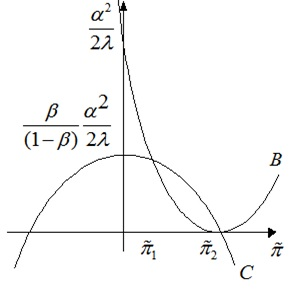
\includegraphics[width=0.9\linewidth]{pic1.jpg} 
		\caption{$\beta < \frac{1}{2}$}
		\label{fig:pic1}
	\end{subfigure}
	\begin{subfigure}{0.5\textwidth}
		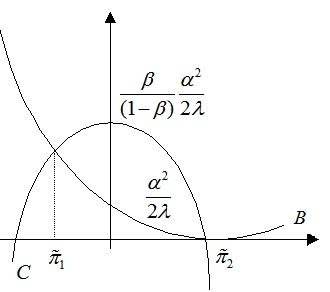
\includegraphics[width=0.9\linewidth]{pic2.jpg}
		\caption{$\beta > \frac{1}{2}$}
		\label{fig:pic2}
	\end{subfigure}
	
	\caption{Графіки втрат і виграшу}
	\label{fig:image2}
\end{figure}

Якщо політик обманює очікування громадськості в нульовий момент часу, то виграш він отримує за рахунок того, що в нульовий момент часу не виправдав сподівань громадськості, а програш - що в подальшому громадськість перестає йому довіряти і завжди чекає більший рівень інфляції, ніж було оголошено.
\\

Отже, виграш обманюючого населення в нульовий момент часу політика
\begin{equation}
B=w^{deception}_0 - w^{fair}_0 = \frac{\lambda\pi^2}{2}+\frac{\alpha^2}{2\lambda}-\alpha\tilde{\pi}
\end{equation}
є квадратичною функцією від декларованого рівня інфляції. Ця функція досягає мінімуму $ B = 0 $ в точці $\tilde{\pi}=\frac{\alpha}{\lambda}$. При $\tilde{\pi}=0$  виграш дорівнює $\frac{\alpha^2}{\lambda}$.

Програш обманюючого населення в нульовий момент часу політика також є квадратичною функцією від декларованого рівня інфляції, оскільки

\begin{equation}
	\label{eq:sec:domain:main4}
C=\sum_{t=1}^{\infty} \beta^t(w^{deception}_t - w^{fair}_t) = -\frac{\lambda\tilde{\pi}^2}{2}+\frac{\alpha^2}{2\lambda}.
\end{equation}



Функція, що задається рівнянням \eqref{eq:sec:domain:main4}, описує параболу,
яка досягає максимуму $C=\frac{\beta}{(1-\beta)}\frac{\alpha^2}{2\lambda} $  в
точцi   $\tilde{\pi}=0$. Значення функції $C$ дорівнює нулю, коли рівень
інфляції становить $\tilde{\pi}\pm\frac{\alpha}{\lambda}$.


Взаєморозміщення графіків втрат і виграшу обманюючого громадськість в нульовий момент часу політика залежить від того, більше чи менше одиниці величина $\frac{\beta}{1-\beta}$.

Якщо   $\frac{\beta}{1-\beta}<1$, то есть  $\beta<\frac{1}{2}$, то функція втрат і функція виграшу перетинаються в точках  $\tilde{\pi}_1>0$ и $\tilde{\pi}_2>0$ \eqref{fig:pic1}, причому  $\tilde{\pi}_1~=~\frac{\alpha(1-2\beta)}{\lambda}$, $\tilde{\pi}_2~=~\frac{\alpha}{\lambda}$. \\
Якщо  $\frac{\beta}{1-\beta}>1,$  тобто  $\beta>\frac{1}{2},$  то функція втрат і функція виграшу перетинаються в точках $\tilde{\pi}_1<0$, $\tilde{\pi}_2>0$ ~(\ref{fig:pic2}).

Таким чином, з проведеного аналізу випливає, що поведінка політика (буде він виконувати обіцянки чи ні) залежить від його відношення до репутації. Якщо для нього репутація не важлива, майбутнє мало впливає на його функцію добробуту $\beta<\frac{1}{2}$, то політику не вигідно вести себе чесно. Оскільки, як видно з \eqref{fig:pic1}, існує досить невисокий рівень інфляції $\tilde{\pi}\in\left(0;\frac{\alpha(1-2\beta)}{\lambda} \right)$ , обіцяючи який він може виграти більше в результаті обману (в порівнянні з чесним поведінкою). Якщо для політика його репутація важлива, майбутнє значимо для його добробуту $\beta<\frac{1}{2}$, то йому має сенс вести себе чесно. Оскільки, як видно з \eqref{fig:pic2}, не існує рівня інфляції близького до нуля, обіцяючи який він може отримати більшу реалізацію своїх цілей в результаті обману в порівнянні з чесною поведінкою.



\subsection{Теоретико-игровая интерпретация модели Барро-Гордона}

В игре участвуют два игрока: $p$ - правительство, $q$ - общественность, которые оперируют инфляцией $\pi$  и индексированием заработной платы $\omega$ соответственно. Для упрощения модели положим, что оба не могут прогнозировать будущие. Каждый игрок выбирает из следующих стратегий: низким $L$  и высоким  $H$ уровнем повышения. В общем виде игра может быть задана в виде матрицы выигрышей, 
\begin{table}[h]
	\centering
	\caption{}
\footnotesize Матрица выигрышей в модели Барро-Гордона\\
\normalsize
\begin{tabular}{|l|l|c|c|}
	\hline
	\multicolumn{2}{|l|}{\multirow{2}{*}{}} & \multicolumn{2}{l|}{Общественность} \\ \cline{3-4} 
	\multicolumn{2}{|l|}{}                  & L                & H                \\ \hline
	\multirow{2}{*}{Правительство}    & L   & a,q              & b,v              \\ \cline{2-4} 
	& H   & c,x              & d,z              \\ \hline
\end{tabular}
\end{table}\\
где параметры $a,b,c,d,q,v,x,z$  - выигрыши удовлетворяющие следующим ограничениям~\cite{libich2008macroeconomic}

\begin{equation}
c>a>d>b, q>v, q\geqslant z>x.
\label{eq:sec:ot:restrictions}
\end{equation}

В данном случае проще всего описать экономику через функцию совокупного предложения Лукаса~\cite{libichIncorpo}

\begin{equation}
\label{eq:sec:ot:lucas}
y_t - Y = \lambda(\pi_t - \omega_t)+\varepsilon_t,
\end{equation}
где  $\lambda>0, y$  – производительность, $Y$ – естественный уровень производительности, а  $\varepsilon$ - макроэкономический шок близкий к нулю. Коэффициенты дисконтирования игроков составляют $\beta_g$ и $\beta_p$, а их функции  полезности  имеют следующий вид 

\begin{equation}
\label{eq:sec:ot:govUtil}
u^g_t=-(\pi_t - \tilde{\pi})^2 + \alpha y_t - \beta(y_t-Y)^2,
\end{equation}

\begin{equation}
\label{eq:sec:ot:pubUtil}
u^p_t=-(\pi_t - \omega)^2,
\end{equation}
где $\tilde{\pi}$ - оптимальный уровень инфляции, а $\alpha > 0, \beta > 0$ описывают относительный вес целей правительства (стабильной инфляции, высокой и стабильной производительности). Общественность озабочена верным ожиданием уровня инфляции для того, чтобы определить уровень зарплат на рынке. 
\\

Так как нас интересует эффект от выбранной политики, то сфокусируемся на долгосрочном исходе игры. Для этого однозначно определим экономику положив $\forall t$,      $\varepsilon_t=0$ , что подразумевает, что мы можем положить $\beta=0$ без потери общности. Из этого следует, что инструмент правительства $\pi$  представляет собой выбор средней инфляции.
\\

В стандартной пошаговой игре, в которой игроки могут менять свое поведение в каждый период, мы используем \eqref{eq:sec:ot:lucas}-\eqref{eq:sec:ot:govUtil} для получения равновесия

\begin{equation}
\label{eq:sec:ot:equilibrium}
\pi^*_t= \tilde{\pi} + \frac{\alpha\lambda}{2}= \omega^*_t,
\end{equation}
что является известным результатом $\pi^*_t > \tilde{\pi}$. Сфокусировав внимание на двух уровнях инфляции мы следуем  ~\cite{ChoiAndMacui96InflationFinancialMarkets}, где были предложены два наиболее естественных варианта – оптимальный уровень из \eqref{eq:sec:ot:govUtil} и согласованного по времени из \eqref{eq:sec:ot:equilibrium}

\begin{equation}
\label{eq:sec:ot:optimal}
\pi \in \left\{L=\tilde{\pi}, H=\tilde{\pi}+\frac{\alpha\lambda}{2} \right\} \ni \omega^*_t.
\end{equation}

Мы можем, учитывая \eqref{eq:sec:ot:lucas}-\eqref{eq:sec:ot:pubUtil} и поделив на $\left(\frac{\alpha\lambda}{2}\right)$,  без потери общности вывести соответствующие выигрыши, представленные в таблице ниже. Так же вне зависимости от $\lambda$ и  $\alpha$ справедливы следующие ограничения для данной игры в дополнение к изначальным~(\ref{eq:sec:ot:restrictions})

\begin{equation}
	\label{eq:sec:ot:constraint}
	c>a=0 > d > b,c=-d=-\frac{b}{2}, q>v,q\geqslant z>x
\end{equation}

\begin{equation}
\label{eq:sec:ot:exampleConstraint}
c=1 > a=0 > d=-1 > b=-2, q=z=0 > v=x=-1,
\end{equation}

\begin{table}[h]
	\centering
	
	\caption{}	
	\footnotesize Матрица выигрышей из~(\ref{eq:sec:ot:exampleConstraint})\\
	\normalsize
\begin{tabular}{|l|l|c|c|}
	\hline
	\multicolumn{2}{|l|}{\multirow{2}{*}{}} & \multicolumn{2}{l|}{Общественность} \\ \cline{3-4} 
	\multicolumn{2}{|l|}{}                  & L                & H                \\ \hline
	\multirow{2}{*}{Правительство}    & L   & 0, 0             & -1,-1            \\ \cline{2-4} 
	& H   & $\frac{1}{2}$,-1             & $-\frac{1}{2}$, 0            \\ \hline
\end{tabular}
		
	\label{table:sec:ot:real}
\end{table}


Стандартная пошаговая игра имеет уникальное равновесие по Нэшу $(H,H)$. Однако, оно неэффективно, так как является Парето доминированным. Это означает, что существует такой исход игры, который улучшит состояние одного, но при этом не ухудшит его для других игроков. В данном случае это «не Нэшовский» исход $(L,L)$.  У правительства возникает соблазн создать неожиданную инфляцию, чтобы повысить производительность и снизить уровень безработицы. Так как общественность рациональна, то будет ожидать высокую инфляцию – оба игрока будут в проигрыше. 


\subsection{Устойчивость равновесных стратегий в модели Барро-Гордона на
	временных шкалах} 

Рассмотрим игровую интерпретацию модели Барро-Гордона на временных шкалах.

Все допущения выдвинутые в стандартной игре остаются. Расширим их:
\begin{itemize}
	\item игра начинается одновременным ходом, 
	\item заранее известно неизменное количество ходов $r^g \in \mathbb{N}$ и $r^p \in \mathbb{N}$,
	\item игра заканчивается через $T$ периодов, где $T$ - наименьшее общее кратное для $r^g$ и $r^p$,
	\item игроки рациональны, обладают равноценными знаниями и полной информацией о структуре игры, матрице выигрышей и всех предыдущих ходах.
\end{itemize}

Другими словами определяется три временных шкалы: правительства, общественности и самой игры:
\begin{equation}
\label{eq:sec:tech:scales}
T_g = \{0,r^g,2r^g,...,T\}, T_p=\{0,r^p,2r^p,...,T\}, T=T_g\cup T_p 
\end{equation}

Главным преимуществом использования однородных временных шкал является экономическая интерпретация: $r^g$ и $r^p$ представляют собой степень возможности изменений политики относительно инфляции и степень реагирования для внесения изменений в заработные платы.
\\

Асинхронная игра на временных шкалах будет как правило иметь несколько равновесий по Нэшу, среди которых мы выберем лучшую в зависимости от под-игры.

\begin{theorem}
	Рассмотрим общую несогласованную по времени игру на однородных временных шкалах, для которой выполняются~(\ref{eq:sec:ot:constraint}) и ~(\ref{eq:sec:tech:scales}). Тогда все SNPE игры будут SNPE Рамсея, если и только если
	
	\begin{equation}
	\label{eq:sec:tech:theoremSystem}
	r^g> \bar{r^g}(R) = \left\{ 
	\begin{aligned} 
	&\frac{c - d}{a-d}r^p= \frac{a-b}{a-d}r^p, &&\text{если } R=0
	\\
	&\frac{(1+R)(c-d)}{a-d}r^p= \frac{a-b + R(c-d)}{a-d}r^p, &&\text{если } 	R\in(0; \bar{R})
	\\
	&\frac{c-d-(1-R)(a-b)}{a-d}r^p= \frac{(a-b)}{a-d}Rr^p, &&\text{если } 	R\in(\bar{R};1)
	\end{aligned}
	\right.		
	\end{equation}
\end{theorem}
где $\bar{R}=\frac{q-v}{z-x+q-v}$. В несогласованной игре, где справедливо ~(\ref{eq:sec:ot:constraint}),  ~(\ref{eq:sec:tech:theoremSystem}) преобразуется в 

\begin{equation}
\frac{r^g}{r^p} \in \left(\frac{3}{2}, 2\right)\cup \left(\frac{5}{2}, \infty\right)
\end{equation}
Доказательство: смотреть Либиха и Штелиха~\cite{libichIncorpo}.


Можно утверждать, что действия игроков могут не всегда быть детерминистическими и/или что частота их ходов различается во времени или подчиняется некоторому случайному процессу. Разнородные временные шкалы позволяют изучать подобные случаи. Для большей эффективности нормализуем горизонт планирования как $T = r^g$. Как и ранее игроки $g$ и $p$ ходят одновременно в первом периоде и во всех $T = r^g$ периодах, в промежутках между которыми общественность так же способна реагировать на ход правительства. Для удобства сравнения оставим все предположения предыдущего параграфа неизменными.

Рассмотрим произвольную временную шкалу $\mathbb{T}$ и произвольную невозрастающую функцию реакции общественности $f : \mathbb{T} \to [0,1]$. В данной работе рассматриваются два представляющих интерес особых случая. В первом, при разнородной (атомистической) общественности, функция реакции может быть интерпретирована как часть общественности, которая уже имела возможность совершить ход. Во втором, при вероятностных ходах общественности, функция реакции может быть интерпретирована как кумулятивная функция распределения её ходов.

Чтобы удостовериться в том, что все SPNE являются SPNE Рамсея, достаточно показать, что в первом ходе оптимальной стратегией $g$ является $L$ вне зависимости от хода общественности в первом периоде. Получим два соответствующих условия:
\begin{equation}
\label{sec:hetero:main1}
ar^g > c \int_0^{r^g} 1 - f(t) \Delta t + d  \int_0^{r^g} f(t) \Delta t ,
\end{equation}
\begin{equation}
\label{sec:hetero:main2}
dr^g > b \int_0^{r^g} 1 - f(t) \Delta t + a  \int_0^{r^g} f(t) \Delta t .
\end{equation}

\begin{theorem}
	\label{spneTh}
	Рассмотрим общую несогласованную по времени игру, в которой выполняется~\eqref{eq:sec:ot:constraint} и $f : \mathbb{T} \to [0,1]$ -- невозрастающая функция реакции. Тогда все SPNE игры являются SPNE Рамсея тогда и только тогда, когда выполняется неравенство
	\begin{equation}
	\label{sec:hetero:main3}
	\int_0^{r^g} f(t) \Delta t > \frac{r^g}{2} .
	\end{equation}
\end{theorem}

Для лучшей наглядности теоремы~\ref{spneTh} и лучшего понимания приведём несколько следствий и рассмотрим пример. Как уже было указано ранее, мы концентрируемся на двух случаях: разнородной общественности и вероятностных моделях.

\subsubsection{Разнородная общественность.} Во-первых, предположим, что существует $N$ различных общественных групп (профсоюзов) $p_1,...,p_N$ с соответствующими $r^{p_1},...,r^{p_N}$ и размерами $s_1,...,s_N \in [0,1]$, которые удовлетворяют естественному предположению $\sum_{i=1}{N}s_i = 1$. Чтобы свести наше внимание к первому ходу правительства, предположим что $r^g$ является кратным для $r^{p_i}$ для всех $i = 1,...,N$, то есть
$$ \frac{r^g}{r^{p_i}} \in \mathbb{N}.$$
Для более асинхронных случаев  см.~\cite{libichIncorpo}. Для данного особого случая теорему~\ref{spneTh} можно переписать следующим образом.\\
\textbf{Следствие 1.} \textit{Рассмотрим общую несогласованную по времени игру, в которой выполняется~\eqref{eq:sec:ot:constraint} и общественность состоит из $N$ различных групп. Тогда все SPNE игры являются SPNE Рамсея тогда и только тогда, когда выполняется неравенство
	\begin{equation}
	\label{sec:hetero:main4}
	\sum_{i=1}^N s_i(r^g - r^{p_i}) \geqslant \frac{r^g}{2} .
	\end{equation}
}
%опять же доказательство

\subsubsection{Вероятностная модель.}
Вернёмся к случаю с унифицированной общественностью, чтобы рассмотреть вероятностные ходы отдельно от влияния эффектов разнородной общественности. В зависимости от результатов переговоров общественность будет реагировать на первый ход правительства в какой-то момент времени из интервала $[a,b], 0< a < b < r^g$, с равномерно распределённым вероятностным законом. Теорема~\ref{spneTh} принимает вид:\\
\textbf{Следствие 2.} \textit{Рассмотрим общую несогласованную по времени игру, в которой выполняется~\eqref{eq:sec:ot:constraint} и общественность делает второй ход в какой-то момент времени из интервала $[a,b]$ с равномерно распределённым вероятностным законом. Тогда все SPNE игры являются SPNE Рамсея тогда и только тогда, когда выполняется неравенство
	\begin{equation}
	\label{sec:hetero:main5}
	\frac{b^2 - a^2}{2} \geqslant b - \frac{r^g}{2} .
	\end{equation}
}
Очевидно, что можно рассматривать произвольные комбинации описанных выше подходов, то есть разнородных игроков с вероятностными ходами, вероятность которых может быть описана некоторыми функциями распределения. Приведём пример.\\
\textbf{Пример 1.} Рассмотрим экономику с двумя профсоюзами, каждый их которых состоит из $s_1$ и $s_2$ рабочих соответственно, так что выполняется $s_1 + s_2 = 1$. Примем в качестве одного периода квартал (раз в квартал выпускаются сводки по макроэкономике). Предположим, что $r^g = 5$ и что время реакции профсоюзов составляют как минимум  1 и 3 квартала, но как максимум -- 1,5 и 3,5 квартала соответственно. Для простоты предположим, что решение, принятое за полтора квартала подчиняется равномерному закону распределения. Тогда получим:
$$ \mathbb{T} :={0} \cup [1, 1.5] \cup {r^g} ,$$
$$ \mathbb{T} :={0} \cup [3, 3.5] \cup {r^g} .$$
Функция реакции тогда имеет вид $f : \mathbb{T}_1\cup\mathbb{T}_2\to[0,1]$:
$$ f(x)\left\{  
\begin{array}{l c l}
0 & if & x = 0,\\
2s_1(x - 1) & if & x \in [1,1.5],\\
s_1 + 2s_2(x - 3) & if & x \in [3,3.5],\\
1 & if & x = 5.
\end{array} 
\right.$$
Интегрируя по $\mathbb{T}_1\cup\mathbb{T}_2$ получим
$$ \int_0^5 f(x) \Delta x = \frac{15}{4}s_1 + \frac{7}{4}s_2. $$
Предположение~\eqref{sec:hetero:main3} теоремы~\ref{spneTh} удовлетворяется (и следовательно единственное равновесие является равновесием Рамсея) тогда и только тогда, когда выполняется
$$ s_1 \geqslant \frac{3}{8}, \text{или, что эквивалентно,} s_2 \leqslant \frac{5}{8}. $$
Интуитивно понятно, что профсоюз, принимающий решения быстрее, должен быть достаточно велик для того, чтобы общая реакция общественности была достаточно быстрой, чтобы препятствовать увеличению инфляции правительством.

\subsection{Классическая модель профсоюз---монополист}
\label{sec:monopoly}

Данная модель является моделью отношений профсоюз---фирма по
Леонтьеву~\cite{LeontiefW}, в которой профсоюз задаёт уровень заработной платы $W$,
после чего фирма выбирает желаемое количество наёмных работников (уровень
найма) $E$. Предполагается, что фирма оперирует в условиях конкурентного рынка с
рыночной ценой $P$.

Функция полезности профсоюза имеет вид 
$$ 
	U = U(W,E), 
	\quad 
		\frac{\partial U}{\partial W} > 0; 
	\quad 
		\frac{\partial U}{\partial E}~>~0;
	\quad   
		\frac{\partial^2 U}{\partial W^2} \leqslant 0.
$$ 
В простейшем случае можно взять, например, $U = \lambda WE$, где $\lambda \in (0; 1)$.

Полезность для фирмы измеряется как прибыль 
$$
	\Pi~=~PY(\bar K,E)~-~WE,
$$ 
где цена $P$ дана, а капитал $\bar K$ фиксирован. Отсюда мы можем переписать 
$$
	\Pi(W,E)~=~R(E)~-~WE,
$$ 
где $R$ --- доход.

Классическим является решение методом обратной индукции.
При этом вначале фирма максимизирует свою прибыль по $E$, считатя уровень
заработной платы фиксированным и заданным. Условие экстремума первого порядка примет вид 
$$ 
	W = R'(E).
$$
Разрешая уравнение относительно $E$, мы получим кривую спроса на рабочую силу: $E~=~g(W)$.
Зная, к чему приходит фирма, профсоюз решает задачу
$$ 
	\max_W U(W,E) = U(W, g(W)).
$$

Схематически решение представлено на графике~\ref{fig:monopoly_union}.
Графически можно показать, что исход игры неэффективен. Точка $X$ является
точкой равновесия обратной индукции модели монополии профсоюза. Точки в
закрашенной области предпочтительнее по Парето, чем $X$. $AB$ является так называемой 
кривой контракта, состоящей из точек, в которых изопрофиты и кривые безразличия
профсоюза имеют общий тангенс~\cite{ShandongUniver}.


\begin{figure}[h]
	\centering
	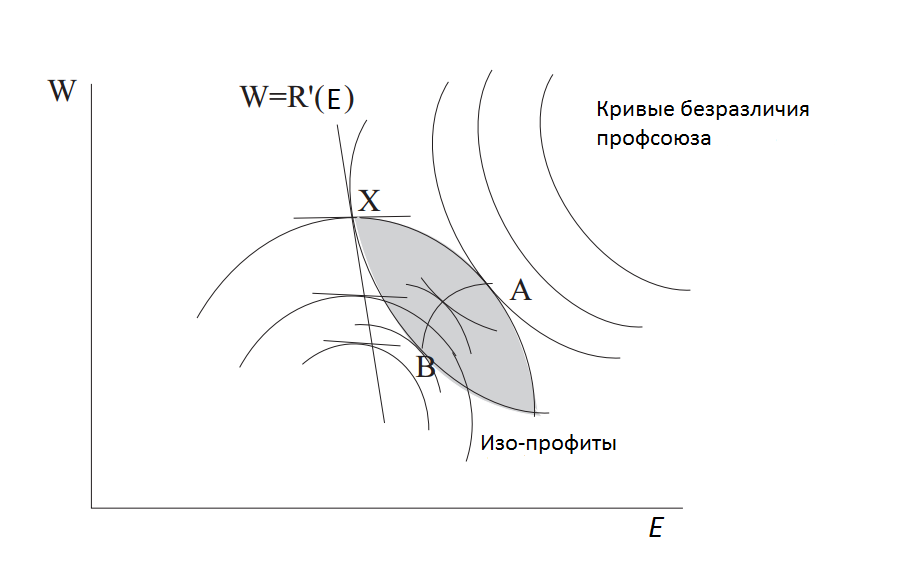
\includegraphics[width=1.0\linewidth]{monopoly_union.png}
	\caption{Кривые безразличия игроков в модели профсоюз---монополист}
	\label{fig:monopoly_union}
\end{figure}

\subsection{Модель профсоюз---монополист на временных шкалах}
Эта модель в литературе не встречается и исследована нами впервые.  
В игре, также как и в непрерывной модели, два игрока: профсоюз $P$ и фирма--монополист
$F$, чьими рычагами влияния на игру являются $W$ (зарплата рабочего) и $E$ 
(количество нанятых рабочих) соответственно.  Каждый игрок выбирает одну из двух
стратегий: установить низкое $L$ или высокое $H$ значение управляемого им параметра. 
В общем виде игра может быть задана следующей матрицей выигрышей: 

\begin{table}[h]
	\centering
	\caption{}
		\footnotesize Матрица выигрышей для модели "профсоюз---монополист"\\
		\normalsize
	\begin{tabular}{|l|l|l|l|}
		\hline
		\multicolumn{2}{|l|}{\multirow{2}{*}{}} & \multicolumn{2}{l|}{Профсоюз} \\ \cline{3-4} 
		\multicolumn{2}{|l|}{}                  & $L$            & $H$            \\ \hline
		\multirow{2}{*}{Фирма}     & $L$     & $a,q$          & $b,v$          \\ \cline{2-4} 
		& $H$     & $c,x$          & $d,z$          \\ \hline
	\end{tabular}
	\label{tab:mono:prof}
\end{table}
Функцию полезности профсоюза мы полагаем линейной: $U(W,E)=\lambda WE$, где $\lambda \in(0;1)$:
$$
	\frac{\partial U}{\partial W} > 0; 
	\quad 
	\frac{\partial U}{\partial E}~>~0 ; 
	\quad
	\frac{\partial^2 U}{\partial W^2} \leqslant 0
$$

$$
	U(0,E) = U(W,0) = U(0,0) = 0.
$$

Функция полезности фирмы иммет вид $\Pi(W,E)=cP(\bar{K},E)-WE$:
$$P(\bar{K}, E)=A\bar{K}^\alpha E^\beta,$$ 
где $A$ --- коэффициент нейтрального технического прогресса, $\alpha$ и $\beta$
--- коэффициенты эластичности валового внутреннего продукта по капитальным и
трудовым затратам.

Для профсюза соотношения между значениями функции полезности для различных игровых ситуаций
будут следующими:
\begin{equation}
U(L,L) < U(L,H) \nsim U(H, L) < U(H,H).
\end{equation}
Соотношение $U(L,H) \nsim U(H, L)$ не может быть определенно однозначно, так
как это <<политический>> выбор между двумя альтернативами: большее количество
людей, получающих меньшую зарплату (условно <<левый>> подход к распределению
доходов) или меньшее количество людей, получающих большую зарплату (условно
<<правый>> подход). 

Для нахождения соотношений между значениями функции полезности фирмы в разных игровых ситуациях
построим график~\ref{fig:monopoly_union1}.

\begin{figure}[h]
	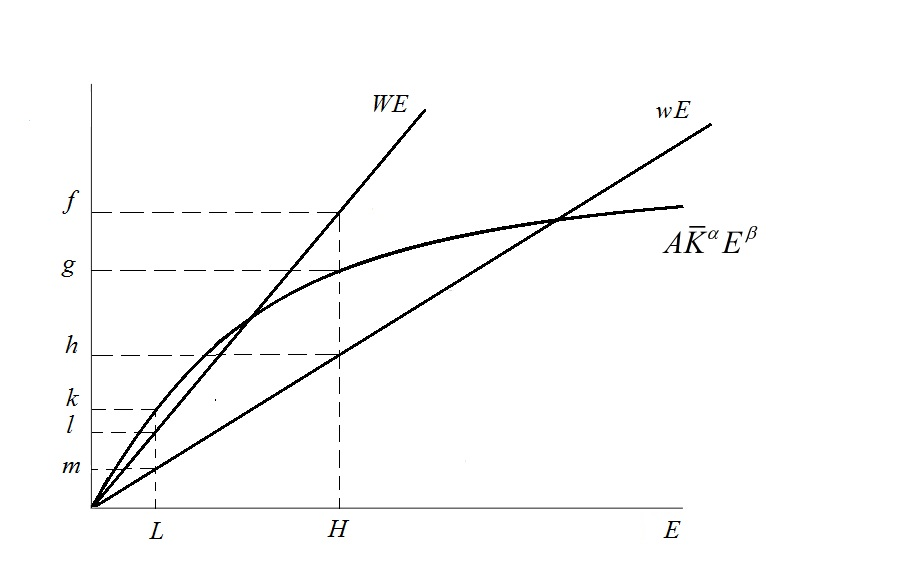
\includegraphics[width=1.0\linewidth]{monopoly_union2.jpg}
	\caption{Компоненты функции полезности фирмы при разных уровнях зарплат}
	\label{fig:monopoly_union1}
\end{figure}

На рисунке $w$ --- низкий уровень зарплат по стратегии $L$, $W$ --- высокий уровень зарплат по стратегии $H$. 
Принимая во внимание, что за исключением количества нанятых и уровня зарплат, все остальные величины постоянны,
легко вывести следующее:
\begin{equation}
\Pi(H,H)=g-f < \Pi(H,L)=k-l < \Pi(L, L)=k-m < \Pi(L,H)=g-h.
\end{equation}
Следовательно матрица выигрышей~(\ref{tab:mono:prof}) будет следующей:
\begin{table}[h]
	
	\centering
	\caption{}
		\footnotesize Матрица выигрышей для модели "профсоюз---монополист"\\
		\normalsize

\begin{tabular}{|l|l|c|c|}
	\hline
	\multicolumn{2}{|l|}{\multirow{2}{*}{}} & \multicolumn{2}{l|}{Профсоюз} \\ \cline{3-4} 
	\multicolumn{2}{|l|}{}                  & L                & H                \\ \hline
	\multirow{2}{*}{Фирма}    & L   & a,q              & b,v              \\ \cline{2-4} 
	& H   & c,x              & d,z              \\ \hline
\end{tabular}
	\label{table:firm}
\end{table}\\
где $q < x \thickapprox v < z, 0 > d < b < a < c$.


%
\section{Дискретные однородные временные шкалы} 

Рассмотрим игровую интерпритацию модели Барро-Гордона на временных шкалах.

Все допущения выдвинутые в стандартной игре остаются. Расширим их:
\begin{itemize}
\item игра начинается одновременным ходом. 
\item заранее известно незименное количество ходов $r^g \in \mathbb{N}$ и $r^p \in \mathbb{N}$.
\item игра заканчивается через $T$ периодов, где $T$ - наименьшее общее кратное для $r^g$ и $r^p$
\item игроки рациональны, обладают равноценными знаниями и полной информацией о структуре игры, матрицей выигрышей, и могут мониторить все предшествующие ходы
 \end{itemize}

Другими словами определяется три временных шкалы: правительства, общественности и самой игры:
\begin{equation}
\label{eq:sec:tech:scales}
T_g = \{0,r^g,2r^g,...,T\}, T_p=\{0,r^p,2r^p,...,T\}, T=T_g\cup T_p 
\end{equation}

Главным преимуществом использования однородных временных шкал это экономическая интерпретация: $r^g$ и $r^p$ представляют собой степень приверженности (???) правительства и степень жесткости поднятия заработных плат общественности (????).

%\section{Разнородные временные шкалы}
\label{sec:hetero}

Можно утверждать, что действия игроков могут не всегда быть детерминистичны и/или что частота их ходов различается во времени или подчиняется некоторому случайному процессу. Разнородные временные шкалы позволяют изучать подобные случаи. Для большей эффективности нормализуем горизонт планирования как $T = r^g$. Как и ранее игроки $g$ и $p$ ходят одновременно в первом периоде и во всех $T = r^g$ периодах, в промежутках между которыми общественность так же способна реагировать на ход правительства. Для удобства сравнения оставим все предположения предыдущего параграфа неизменными.

Рассмотрим произвольную временную шкалу $\mathbb{T}$ и произвольную невозрастающую функцию реакции общественности $f : \mathbb{T} \to [0,1]$. В данной работе рассматриваются два представляющих интерес особых случая. В первом, при разнородной (атомистической) общественности, функция реакции может быть интерпретирована как часть общественности, которая уже имела возможность совершить ход. Во втором, при вероятностных ходах общественности, функция реакции может быть интерпретирована как кумулятивная функция распределения её ходов.

Чтобы удостовериться в том, что все SPNE являются SPNE Рамси, достаточно показать, что в первом ходе оптимальной стратегией $g$ является $L$ вне зависимости от хода общественности в первом периоде. Получим два соответствующих условия:
\begin{equation}
\label{sec:hetero:main1}
ar^g > c \int_0^{r^g} 1 - f(t) \Delta t + d  \int_0^{r^g} f(t) \Delta t ,
\end{equation}
\begin{equation}
\label{sec:hetero:main2}
dr^g > b \int_0^{r^g} 1 - f(t) \Delta t + a  \int_0^{r^g} f(t) \Delta t .
\end{equation}

\begin{theorem}
\label{spneTh}
  Рассмотрим общую несогласованную по времени игру, в которой выполняется~\eqref{eq:sec:ot:constraint} и $f : \mathbb{T} \to [0,1]$ -- невозрастающая функция реакции. Тогда все SPNE игры являются SPNE Рамси тогда и только тогда, когда выполняется неравенство
\begin{equation}
\label{sec:hetero:main3}
\int_0^{r^g} f(t) \Delta t > \frac{r^g}{2} .
\end{equation}
\end{theorem}

Для лучшей наглядности теоремы~\ref{spneTh} и лучшего понимания приведём несколько следствий и рассмотрим пример. Как уже было указано ранее, мы концентрируемся на двух случаях: разнородной общественности и вероятностных моделях.

\subsection{Разнородная общественность.} Во-первых, предположим, что существует $N$ различных общественных групп (профсоюзов) $p_1,...,p_N$ с соответствующими $r^{p_1},...,r^{p_N}$ и размерами $s_1,...,s_N \in [0,1]$, которые удовлетворяют ествественному предположению $\sum_{i=1}{N}s_i = 1$. Чтобы свести наше внимание к первому ходу правительства, предположим что $r^g$ является кратным для $r^{p_i}$ для всех $i = 1,...,N$, то есть
$$ \frac{r^g}{r^{p_i}} \in \mathbb{N}.$$
Для более асинхронных случаев  см.~\cite{libichIncorpo}. Для данного особого случая теорему~\ref{spneTh} можно переписать следующим образом.\\
\textbf{Следствие 1.} \textit{Рассмотрим общую несогласованную по времени игру, в которой выполняется~\eqref{eq:sec:ot:constraint} и общественность состоит из $N$ различных групп. Тогда все SPNE игры являются SPNE Рамси тогда и только тогда, когда выполняется неравенство
\begin{equation}
\label{sec:hetero:main4}
\sum_{i=1}^N s_i(r^g - r^{p_i}) \geq \frac{r^g}{2} .
\end{equation}
}
%опять же доказательство

\subsection{Вероятностная модель.}
Вернёмся к случаю с унифицированной общественностью, чтобы рассмотреть вероятностные ходы отдельно от влияния эффектов разнородной общественности. В зависимости от результатов переговоров общественность будет реогировать на первый ход правительства в какой-то момент времени из интервала $[a,b], 0< a < b < r^g$, с равномерно распределённым вероятностным законом. Теорема~\ref{spneTh} принимает вид:\\
\textbf{Следствие 2.} \textit{Рассмотрим общую несогласованную по времени игру, в которой выполняется~\eqref{eq:sec:ot:constraint} и общественность делает второй ход в какой-то момент времени из интервала $[a,b]$ с равномерно распределённым вероятностным законом. Тогда все SPNE игры являются SPNE Рамси тогда и только тогда, когда выполняется неравенство
\begin{equation}
\label{sec:hetero:main5}
\frac{b^2 - a^2}{2} \geq b - \frac{r^g}{2} .
\end{equation}
}
Очевидно, что можно рассматривать произвольные комбинации описанных выше подходов, то есть разнородных игроков с вероятностными ходами, вероятность которых может быть описана некоторыми функциями распределения. Приведём пример.\\
\textbf{Пример 1.} Рассмотрим экономику с двумя профсоюзами, каждый их которых состоит из $s_1$ и $s_2$ рабочих соответственно, так что выполняется $s_1 + s_2 = 1$. Примем в качестве одного периода квартал (раз в квартал выпускаются сводки по макроэкономике). Предположим, что $r^g = 5$ и что время реакции профсоюзов составляют как минимум  1 и 3 квартала, но как максимум -- 1,5 и 3,5 квартала соответственно. Для простоты предположим, что решение, принятое за полтора квартаала подчиняется равномерному законц распределения. Тогда получим:
$$ \mathbb{T} :={0} \cup [1, 1.5] \cup {r^g} ,$$
$$ \mathbb{T} :={0} \cup [3, 3.5] \cup {r^g} .$$
Функция реакции тогда имеет вид $f : \mathbb{T}_1\cup\mathbb{T}_2\to[0,1]$:
$$ f(x)\left\{  
\begin{array}{l c l}
0 & if & x = 0,\\
2s_1(x - 1) & if & x \in [1,1.5],\\
s_1 + 2s_2(x - 3) & if & x \in [3,3.5],\\
1 & if & x = 5.
\end{array} 
\right.$$
Интегрируя по $\mathbb{T}_1\cup\mathbb{T}_2$ получим
$$ \int_0^5 f(x) \Delta x = \frac{15}{4}s_1 + \frac{7}{4}s_2. $$
Предположение~\eqref{sec:hetero:main3} теоремы~\ref{spneTh} удовлетворяется (и cледовательно единственное равновесие является равновесием Рамси) тогда и только тогда, когда выполняется
$$ s_1 \geq \frac{3}{8}, \text{или, что эквивалентно,} s_2 \leq \frac{5}{8}. $$
Интуитивно понятно, что профсоюз, принимающий решения быстрее, должен быть достаточно велик для того, чтобы общая реакция общественности была достаточно быстрой, чтобы препятствовать увеличению инфляции правительством.

%\section{Модель монополии профсоюза}
\label{sec:monopoly}

Данная модель является моделью отношений профсоюз-фирма по Леонтьеву~\cite{LeontiefW}, в которой профсоюз задаёт уровень заработной платы, после чего фирма выбирает желаемое количество наёмных работников (уровень найма). Предположим что фирма оперирует в условиях конкурентного рынка с рыночной ценой $P$.\\

Порядок игры следующий:\\
\textbf{Первый этап.} Профсоюз устанавливает уровень заработной платы $W$.
\textbf{Второй этап.} Фирма выбирает уровень найма $E$.\\

Выигрыши составляют:\\
Функция полезности профсоюза имеет вид 
$$ U = U(W,E), \quad \frac{\partial U}{\partial W} > 0; \quad \frac{\partial U}{\partial E}~>~0.$$ 
Например $U = \lambda WE.$, где $\lambda \in (0; 1)$\\
Полезность для фирмы измеряется как прибыль 
$$\Pi~=~PY(\bar K,E)~-~WE,$$ 
где цена $P$ дана, а капитал $\bar K$ фиксирован. Отсюда мы можем переписать 
$$\Pi(W,E)~=~R(E)~-~WE,$$ 
где $R$ -- доход.\\

Решение методом обратной индукции:\\
\textbf{Второй этап.} Фирма максимизирует свою прибыль по $E$ при заданном уровне заработной платы. Условие первого порядка примет вид
$$ W = R'(E) = MPE. $$
Разрешая относительно $E$ получим кривую спроса: $E~=~g(W)$.\\
\textbf{Первый этап.} Решается
$$ \max_W U(W,E) = U(W,g(W)). $$
Решение приведено на графике~\ref{fig:monopoly_union}. Графически можно показать, что исход игры неэффективен. Точка $X$ является точкой равновесия обратной индукции модели монополии профсоюза. Точки в закрашенной области Парето-предпочтительнее $X$. $AB$ является кривой контракта, состоящей из точек, в которых изо-профиты и кривые безразличия профсоюза имеют общий тангенс~\cite{ShandongUniver}.


\begin{figure}[h]
		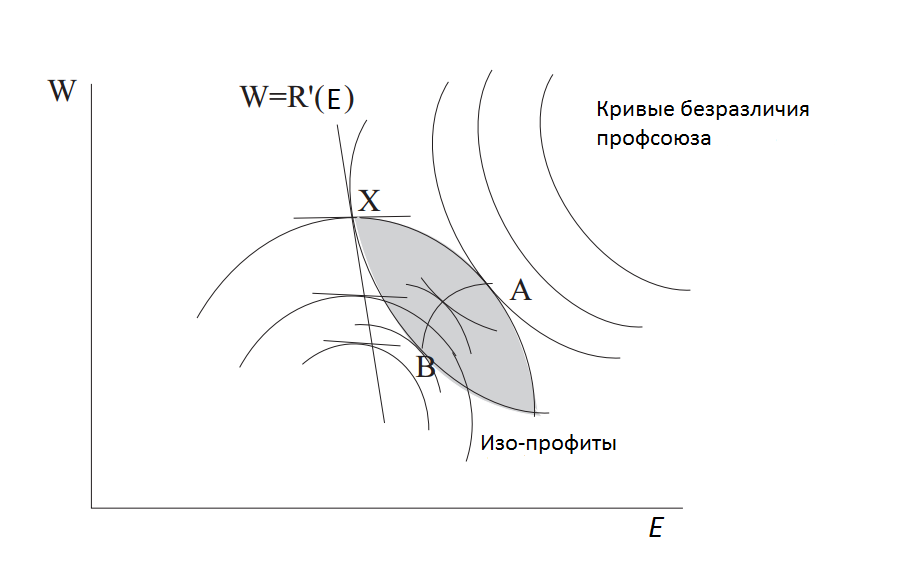
\includegraphics[width=1.0\linewidth]{monopoly_union.png}
		\caption{}
		\label{fig:monopoly_union}
\end{figure}




%\section{Модель монополии профсоюза на временных шкалах}

В игре, как и в непрерывной модели присутсвует два игрока: профсоюз $P$ и фирма $F$, чьими рычагами влияния на игру являются $W$ - зарплата рабочего и $E$ - количество нанятых рабочих соответственно.
Каждый игрок выбирает из следующих стратегий: низким $L$ и высоким $H$ уровнем повышения. В общем виде игра может быть задана следующей матрицей выигрышей: 

\begin{table}[h]
	\centering
	\begin{tabular}{|l|l|l|l|}
		\hline
		\multicolumn{2}{|l|}{\multirow{2}{*}{}} & \multicolumn{2}{l|}{Union} \\ \cline{3-4} 
		\multicolumn{2}{|l|}{}                  & $L$            & $H$            \\ \hline
		\multirow{2}{*}{Firm}     & $L$     & $a,q$          & $b,v$          \\ \cline{2-4} 
		& $H$     & $c,x$          & $d,z$          \\ \hline
	\end{tabular}
\end{table}  

Функция полезности профсоюза  $U_t(W,E)=\lambda WE$, где $\lambda \in(0;1)$:
$$\frac{\partial U}{\partial W} > 0; \quad \frac{\partial U}{\partial E}~>~0 \quad U(0,E)=U(W,0)=U(0,0)=0,$$
при этом 
$$U(L,L) < U(L,H) \le U(H, L) < U(H,H) $$

Функция полезности фирмы $\Pi_t(W,E)=cP(\bar{K},E)-WE$:
$$P(\bar{K}, E)=A\bar{K}^\alpha E^\beta$$, где $A$ – коэффициент нейтрального технического прогресса, $\alpha$ и $\beta$ – коэффициенты эластичности валового внутреннего продукта по капитальным и трудовым затратам.\\

$$\Pi(L,L)>\Pi(H,L)$$
$$\Pi(H,H)<\Pi(L,H)$$

Алексей Павлович, не могу понять, как можно вывести единое правило, если всё зависет от разных коэффициентов, ведь соотношение между функциями зависят от того, какое слогаемое из $\Pi_t(W,E)=cP(\bar{K},E)-WE$ растет быстрее.

%\section{Программная реализация} 

\subsection{Информация о программе}
В рамках дипломной работы была разработана программа, которая эмулирует биматричную игру на временных шкалах и доказывает эмпирически изложенные в работе результаты. 
\\

Разработка программного продукта велась на языке Python 3.4.
Программа позволяет пользователю задать $r^g$, $r^p$ и соответствующие скалярные функции поведения игрока в определенный момент времени. Значениями данной функции будет вероятность выбора игроком  стратегии $H$ в данный период времени. Так же пользователь может задать количество запусков игры с входящими данными для подсчета статистики. В качетсве интерфейса входящих данных был выбран txt файл.

\subsection{Пояснения к коду}
 \begin{lstlisting}[style=csharpinlinestyle]
	 util.fromFileToMap(filepath) 
 \end{lstlisting}
Функция парсит входящие данных

 \begin{lstlisting}[style=csharpinlinestyle]
	 nash.calculate_nash(government_payoffs, public_payoffs)
 \end{lstlisting}
 Функция рассчитывает равновесие по Нэшу для стандартной игры.
 
 
 \begin{lstlisting}[style=csharpinlinestyle]
	 nash.time_scales_game(request, government_payoffs, public_payoffs))
 \end{lstlisting}
 Имитация игры на временных шкалах, результатом который есть вектор выигрышей игроков за время игры
 
  \begin{lstlisting}[style=csharpinlinestyle]
	  util.create_all_stats(array, player_name, time)
  \end{lstlisting}
 Рассчитывает статистические параметры, строит гистограмму для выигрышей одного игрока.
 



\setcounter{forsec}{3}
\section{Примеры} 
\subsection{Барро-Гордон}
Положим, что матрица выигрышей двух игроков соответствует~(\ref{table:sec:ot:real}).\\
\begin{table}[h]
	\centering
	\begin{tabular}{|l|l|l|l|}
		\hline
		\multicolumn{2}{|l|}{\multirow{2}{*}{}} & \multicolumn{2}{l|}{Общественность} \\ \cline{3-4} 
		\multicolumn{2}{|l|}{}                  & $L$            & $H$            \\ \hline
		\multirow{2}{*}{Правительство}     & $L$     & $0,0$          & $-1,-1$          \\ \cline{2-4} 
		& $H$     & $\frac{1}{2},-1$          & $-\frac{1}{2},0$          \\ \hline
	\end{tabular}
	\caption{}	
	\label{table:sec:ot:real1}
\end{table}\\
$r^g= 7 $ - количество ходов совершаемое  правительством за игру\\
$r^p= 4 $ - количество ходов совершаемое  обществом за игру\\

Проверим выполнение условия теоремы~\ref{eq:sec:tech:theoremSystem} для матрицы выигрышей~\ref{table:sec:ot:real1}. 

$$
r^g> \bar{r^g}(R) = \left\{ 
\begin{aligned} 
&2r^p= 2r^p, &&\text{если } R=0
\\
&2(1+R)r^p= 2(1+R)r^p, &&\text{если } 	R\in\left(0; \frac{1}{2}\right)
\\
&2Rr^p= 2Rr^p, &&\text{если } 	R\in\left( \frac{1}{2};1\right)
\end{aligned}
\right.		
$$

$$
r^g> \bar{r^g}(R) = 0$$
$$
4 > 0
$$
Следовательно $\frac{r^g}{r^p} \in \left(\frac{3}{2};2\right)$ выбраны правильно и все совершенные равновесия по под-играм должны быть совершенными равновесиями по под-играм Рамсея. \\
 
\begin{itemize}
\item
Рассмотрим случай, когда правительство скорее склонно ввести высокий уровень инфляции, а общественность предполагая, что правительство пойдет на этот шаг с высокой долей вероятности поднимет зарплаты:\\
$q^g =[ 0.5; 0.9; 0.7; 0.5; 0.9; 0.73; 0.8 ]$ - соответствующая скалярная функция \\
$q^p=[ 0.8; 0.9; 0.8; 1 ] $ - соответствующая скалярная функция \\
С помощью программы проведем эмуляцию 100 игр с такими исходными данными.

\begin{figure}[h]
	\centering
		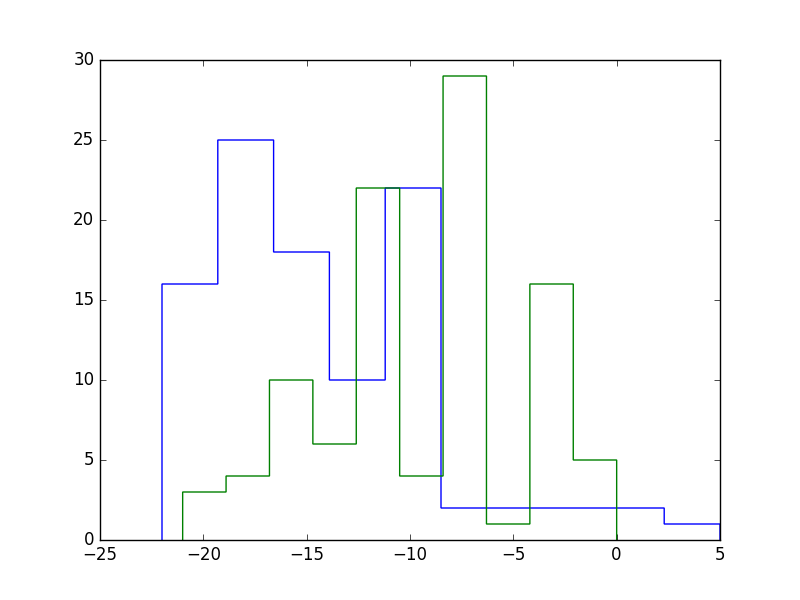
\includegraphics[width=0.5\linewidth]{Public1.png}
			
	\caption{Гистограмма выигрышей, синий - правительство, зеленый - общественность}
	\label{fig:stat1}
\end{figure}

\begin{table}[h]
	\centering
	\begin{tabular}{|l|l|l|}
		\hline
		& Правительство & \multicolumn{1}{c|}{Общественность} \\ \hline
		Среднее                                                           & -14.26       & -9.46                         \\ \hline
		\begin{tabular}[c]{@{}l@{}}Стандартное \\ отклонение\end{tabular} & 5.34       & 4.66                         \\ \hline
		Ассиметрия                                                        & 1.10          & -0.041                          \\ \hline
		Эксцесс                                                           & 1.37        &  -0.37                         \\ \hline
	\end{tabular}
\end{table}

Согласно полученным результатам легко видеть, что подобный набор стратегий невыгоден обеим сторонам, к тому же правительству из-за более "мягкого" подхода "более невыгодно".\\


\item Рассмотрим случай, когда правительство на последнем шаге может отступить от оптимальной для обоих игроков стратегии $(L,L)$.
\\
Для этого положим скалярные функции:\\
$q^g =[ 0; 0; 0; 0; 0; 0; 0.3 ]$ \\
$q^p=[ 0; 0; 0; 0 ] $ \\


\begin{figure}[h]
	

		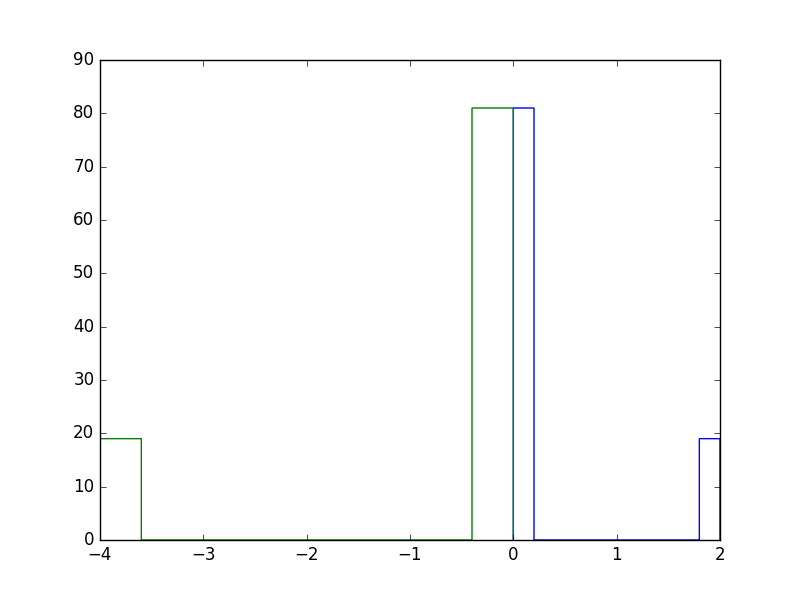
\includegraphics[width=0.5\linewidth]{Public.png}
	\centering	
	\caption{Гистограмма выигрышей, синий - правительство, зеленый - общественность}
	\label{fig:stat}
\end{figure}

\begin{table}[h]
	\centering
	\begin{tabular}{|l|l|l|}
		\hline
		& Правительство & \multicolumn{1}{c|}{Общественность} \\ \hline
		Среднее                                                           & 0.39        & -0.78                         \\ \hline
		\begin{tabular}[c]{@{}l@{}}Стандартное \\ отклонение\end{tabular} & 0.78         & 1.56                          \\ \hline
		Ассиметрия                                                        & 1.6          & -1.11                          \\ \hline
		Эксцесс                                                           & 0.58        & 0.58                        \\ \hline
	\end{tabular}
\end{table}

Данная стратегия является выигрышной для правительства, если общественность не ожидает подобного хода под конец действия срока правительства.\\

\item Рассмотрим случай, когда общественность доверяет правительству и почти уверенно, что оно не может поднять уровень инфляции к окончанию срока своего правления.\\
Для этого положим скалярные функции:\\
$q^g =[ 0; 0; 0; 0; 0; 0; 0.3 ]$ \\
$q^p=[ 0; 0; 0; 0.15] $ \\
	
	\begin{figure}[h]
		
\centering
				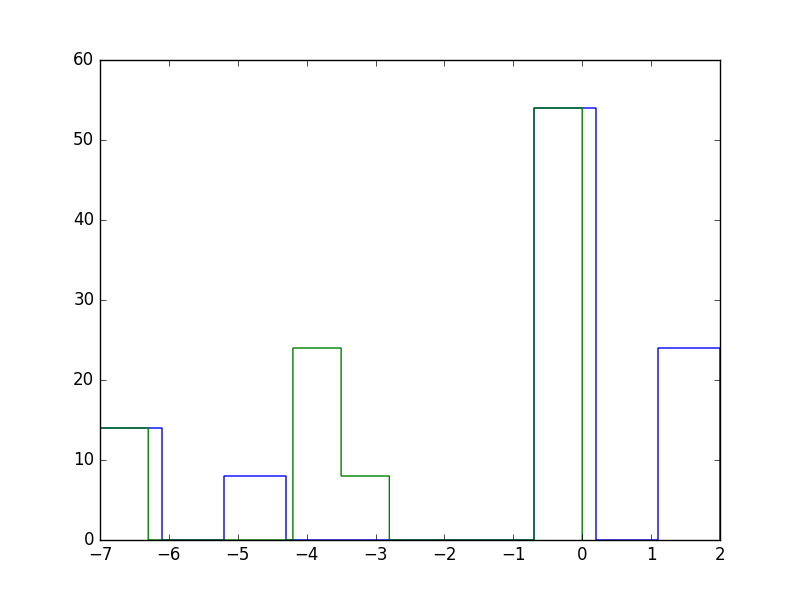
\includegraphics[width=0.5\linewidth]{Public2.png}
		
		\caption{Гистограмма выигрышей, синий - правительство, зеленый - общественность}
		\label{fig:stat2}
	\end{figure}
	\begin{table}[h]
		\centering
		\begin{tabular}{|l|l|l|}
			\hline
			& Правительство & \multicolumn{1}{c|}{Общественность} \\ \hline
			Среднее                                                           & -0.9       &  -2.18                        \\ \hline
			\begin{tabular}[c]{@{}l@{}}Стандартное \\ отклонение\end{tabular} & 3         & 2.58                         \\ \hline
			Ассиметрия                                                        & -1.16          & -0.68                         \\ \hline
			Эксцесс                                                           &  -0.06       & -0.95                        \\ \hline
		\end{tabular}
	\end{table}
	
	
Легко видеть, что данная стратегия однозначно ухудшает позицию правительства, но так же не выгодна общественности.\\


\item Рассмотрим случай, когда общественность не доверяет правительству и почти уверенно, что оно повысит уровень инфляции к окончанию срока своего правления.\\
	 	Для этого положим скалярные функции:\\
	 $q^g =[ 0; 0; 0; 0; 0; 0; 0.3 ]$ \\
	 $q^p=[ 0; 0; 0; 0.8] $ \\
	 
 	\begin{figure}[h]
 		\centering
 			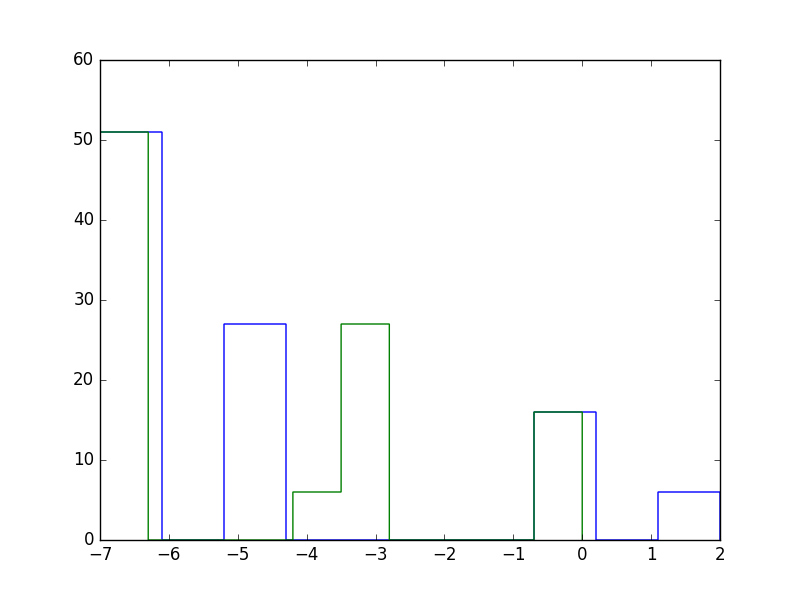
\includegraphics[width=0.5\linewidth]{Public3.png}
 		\caption{Гистограмма выигрышей, синий - правительство, зеленый - общественность}
 		\label{fig:stat3}
 	\end{figure}
 	
 	\begin{table}[h]
 		\centering
 		\begin{tabular}{|l|l|l|}
 			\hline
 			& Правительство & \multicolumn{1}{c|}{Общественность} \\ \hline
 			Среднее                                                           & -4.8      &  -4.62                         \\ \hline
 			\begin{tabular}[c]{@{}l@{}}Стандартное \\ отклонение\end{tabular} &  2.99        &  2.65                          \\ \hline
 			Ассиметрия                                                        & 1.18          &0.54                          \\ \hline
 			Эксцесс                                                           & -0.12       & -1.15                       \\ \hline
 		\end{tabular}
 	\end{table}	

 
 Данная стратегия является равносильно невыгодна для обоих игроков.\\
 
В связи с полученными результатами можно сделать вывод, что если правительство имеет больше шагов на временных шкалах, то ей имеет смысл отклонится от оптимальной по Парето стратегии $L,L$ и повысить уровень инфляции под конец срока своего правления, так как даже если общественность будет ожидать такого хода, то с целью минимизировать свои потери не будет повышать индексирование заработной платы заранее. Естественно если правительство захочет заручиться поддержкой общественности на следующих выборах, то такой ход с её стороны будет сродни "политическому самоубийству".

\end{itemize}
\subsection{Монополия профсоюза}
Положим матрицу выигрышей в соответствии с~\ref{table:firm} следующим образом:
\begin{table}[h]
	
	\centering
	\begin{tabular}{|l|l|l|l|}
		\hline
		\multicolumn{2}{|l|}{\multirow{2}{*}{}} & \multicolumn{2}{l|}{Профсоюз} \\ \cline{3-4} 
		\multicolumn{2}{|l|}{}                  & $L$            & $H$            \\ \hline
		\multirow{2}{*}{Фирма}     & $L$     & $3, 1$          & $2, 3.9$          \\ \cline{2-4} 
		& $H$     & $7, 4$          & $-3, 7$          \\ \hline
	\end{tabular}
	
\end{table}\\
Для нахождения равновесия по Нэшу посчитаем следующее: 
\begin{itemize}
\item Фирма
	$$ L:  3\alpha + 2(1-\alpha)=\alpha + 2$$
	$$ H: 7\alpha - 3(1-\alpha)=10\alpha - 3$$
	
	$$10\alpha - 3 = \alpha+2 $$:
	$$\alpha = \frac{5}{9} $$
	
\item Профсоюз
	
	 $$L: \beta + 4(1-\beta)=-3\beta + 4$$
	 $$H: 3.9\beta + 7(1-\beta)=-3.1\beta +7$$
	$$0.1\beta  = 3 $$
	$$\beta = 30 $$
	
	
\end{itemize}

Следовательно равновесием по Нэшу будет стратегия $L,H$.

В каждом столбце матрицы фирмы найдем максимальный элемент. 
Затем в каждой строке матрицы профсоюза выберем наибольший элемент.
Платежная матрица фирмы:\\
\begin{table}[h]
	\centering
	\begin{tabular}{|l|l|}
		\hline
		3 1 & \textbf{2 3.9}  \\ \hline
		\textbf{7} 4 & -3 \textbf{7} \\ \hline
	\end{tabular}
\end{table}\\
Оптимальной по Парето будет стратегия $(H,L)$.\\
$r^f= 4 $ - количество ходов совершаемое фирмой за игру\\
$r^p= 3 $ - количество ходов совершаемое профсоюзом за игру\\ \\

\begin{itemize}
\item Рассмотрим случай, когда оба игрока стараются следовать равновесной стратегии по Нэшу:\\
$q^f =[ 0.9; 0.9; 0.9; 0.9 ]$ - соответствующая скалярная функция фирмы\\
$q^p=[ 0.1; 0.1; 0.1] $ - соответствующая скалярная функция профсоюза\\

 	\begin{figure}[h]
 		\centering
 		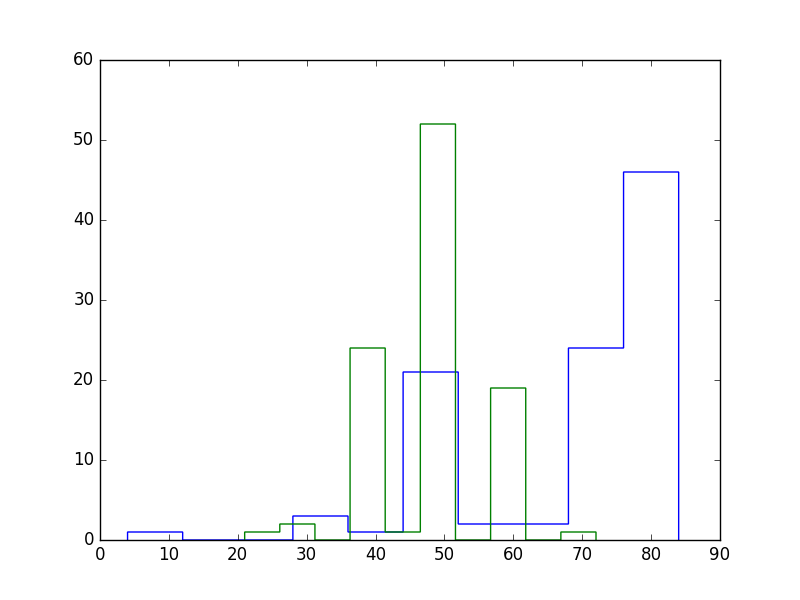
\includegraphics[width=0.5\linewidth]{Public4.png}
 		\caption{Гистограмма выигрышей, синий - фирма, зеленый - профсоюз}
 		\label{fig:stat4}
 	\end{figure}
 	
 	\begin{table}[h]
 		\centering
 		\begin{tabular}{|l|l|l|}
 			\hline
 			& Фирма & \multicolumn{1}{c|}{Профсоюз} \\ \hline
 			Среднее                                                           & 69.02      &  47.84                        \\ \hline
 			\begin{tabular}[c]{@{}l@{}}Стандартное \\ отклонение\end{tabular} & 18.10        &  8.19                          \\ \hline
 			Ассиметрия                                                        & -1.04          &0.017                          \\ \hline
 			Эксцесс                                                           & 0.25        & 0.69                        \\ \hline
 		\end{tabular}
 	\end{table}
 	
 	
 \item Рассмотрим случай, когда профсоюз пытается увеличивать зарплату, на своём последнем шаге, а фирма для выхода из нерентабельного положения сокращает количество сотрудников.\\
 $q^f =[ 0.9; 0.9; 0.9; 0.1 ]$ - соответствующая скалярная функция фирмы\\
 $q^p=[ 0.1; 0.1; 0.9] $ - соответствующая скалярная функция профсоюза\\
 \begin{figure}[h]
 	\centering
 	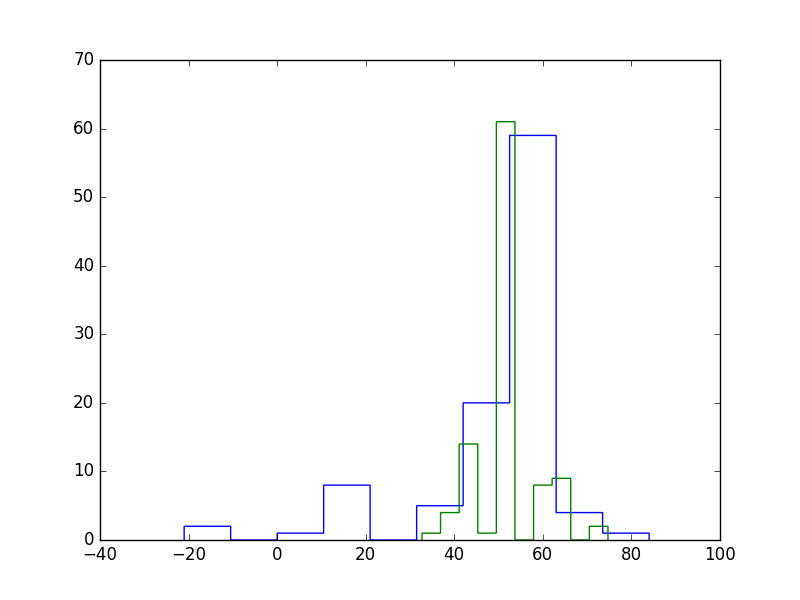
\includegraphics[width=0.5\linewidth]{Public5.png}
 	\caption{Гистограмма выигрышей, синий - фирма, зеленый - профсоюз}
 	\label{fig:stat5}
 \end{figure}
 
 \begin{table}[h]
 	\centering
 	\begin{tabular}{|l|l|l|}
 		\hline
 		& Фирма & \multicolumn{1}{c|}{Профсоюз} \\ \hline
 		Среднее                                                           & 50.48      &  51.1                        \\ \hline
 		\begin{tabular}[c]{@{}l@{}}Стандартное \\ отклонение\end{tabular} & 17.18        &  7.17                          \\ \hline
 		Ассиметрия                                                        & -2.02          &0.57                          \\ \hline
 		Эксцесс                                                           & 5.21        & 1.44                        \\ \hline
 	\end{tabular}
 \end{table}
такая стратегия незначительно улучшит позиции профсоюза, но заметно пошатнет позицию фирмы.

\item Рассмотрим случай, когда профсоюз увеличит зарплату во второй раз и вернется к оптимальной стратегии на третий период:\\
 $q^f =[ 0.9; 0.9; 0.1; 0.9 ]$ - соответствующая скалярная функция фирмы\\
 $q^p=[ 0.1; 0.9; 0.1] $ - соответствующая скалярная функция профсоюза\\
 \begin{figure}[h]
 	\centering
 	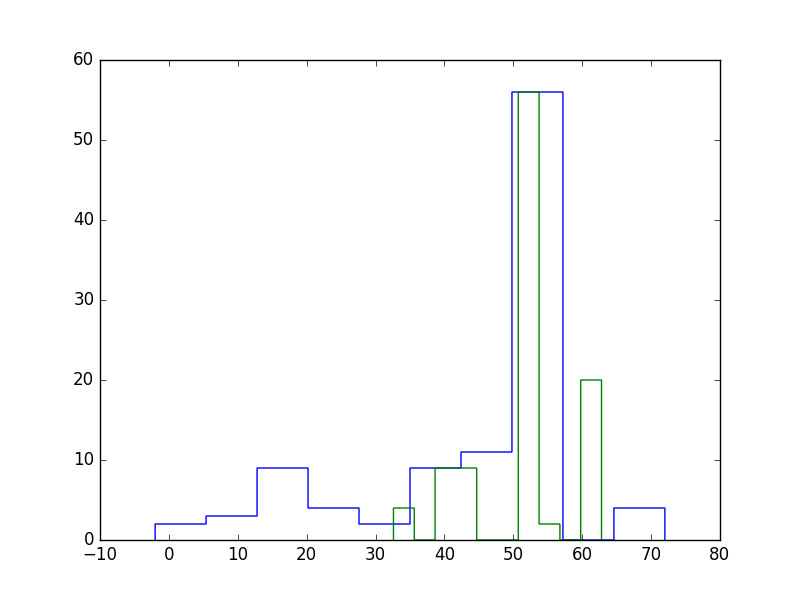
\includegraphics[width=0.5\linewidth]{Public6.png}
 	\caption{Гистограмма выигрышей, синий - фирма, зеленый - профсоюз}
 	\label{fig:stat6}
 \end{figure}
 
 \begin{table}[h]
 	\centering
 	\begin{tabular}{|l|l|l|}
 		\hline
 		& Фирма & \multicolumn{1}{c|}{Профсоюз} \\ \hline
 		Среднее                                                           & 43.06      &  50.64                        \\ \hline
 		\begin{tabular}[c]{@{}l@{}}Стандартное \\ отклонение\end{tabular} & 14.47        &  7.38                          \\ \hline
 		Ассиметрия                                                        & -1.06          &-0.29                          \\ \hline
 		Эксцесс                                                           & 1.30       &0.09                        \\ \hline
 	\end{tabular}
 \end{table}
 
 Снова таки разовая акция поднятия зарплат даёт профсоюзу незначительный выигрыш, но фирма при этом проигрывает относительно много больше, чем выигрывает профсоюз.
 
 \item Рассмотрим случай, когда профсоюз поднимает на втором своём ходе зарплату, но не опускает его вплоть до конца игры:\\ 
 
  $q^f =[ 0.9; 0.9; 0.1; 0.2 ]$ - соответствующая скалярная функция фирмы\\
  $q^p=[ 0.1; 0.9; 0.8] $ - соответствующая скалярная функция профсоюза\\
  \begin{figure}[h]
  	\centering
  	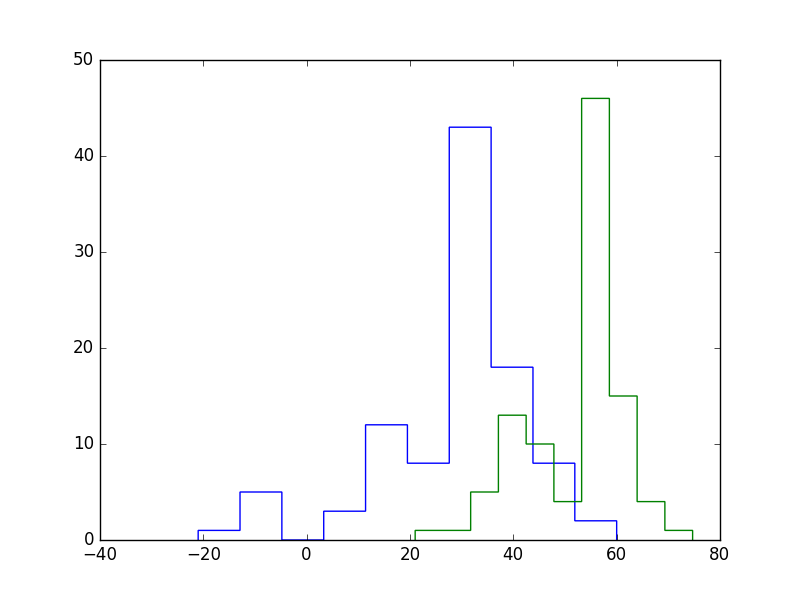
\includegraphics[width=0.5\linewidth]{Public7.png}
  	\caption{Гистограмма выигрышей, синий - фирма, зеленый - профсоюз}
  	\label{fig:stat7}
  \end{figure}
  
  \begin{table}[h]
  	\centering
  	\begin{tabular}{|l|l|l|}
  		\hline
  		& Фирма & \multicolumn{1}{c|}{Профсоюз} \\ \hline
  		Среднее                                                           & 30.37     &  51.37                        \\ \hline
  		\begin{tabular}[c]{@{}l@{}}Стандартное \\ отклонение\end{tabular} & 13.64        &  8.99                          \\ \hline
  		Ассиметрия                                                        & -1.36         &-0.53                          \\ \hline
  		Эксцесс                                                           & 2.74       & 0.8                        \\ \hline
  	\end{tabular}
  \end{table}
  
Фирма снова теряет в относительных деньгах, в то время как профсоюз только незначительно увеличивает своё положение. 
Разумно с точки зрения фирмы сделать предложение профсоюзу не менять уровень зарплат с оптимального, а взамен отплачивать разным видом бонусов. Тогда функция полезности изменится для обоих игроков на равную величину. Фирме стоит подобрать эту величину бонусов так, чтобы остаток между её оптимальным выигрышем после вычитания бонусов был чем-то средним между собственными выигрышами, когда профсоюз устанавливает высокий уровень зарплат и низкий.
\end{itemize}

\sectioncentered*{Выводы}
\addcontentsline{toc}{section}{Выводы}

В данной работе была рассмотрена игровая интерпретация модели Барро-Гордона на
временных шкалах.  Нами впервые введена игровая интерпретация модели <<профсоюз
--- монополист>>. Эта модель была рассмотрена и на временные шкалах.
Разработано программное обеспечение для имитационного моделирования
рассмотренных макроэкономических игр. 

В результате проведенной работы было показано, что на временных шкалах
монополисту стоит договариваться с профсоюзом о дополнительных выплатах
(например, в виде бонусов) при низком уровен найма вместо установления высокого
уровня найма.  В противном случае профсоюз всегда будет устанавливать высокий
уровень зарплат, что невыгодно монополисту, так как он потеряет больше, чем
если бы отдал часть выручки в виде бонусов.



% Зачем: Изменение надписи для списка литературы
% Почему: Пункт 2.8.1 Требований по оформлению пояснительной записки.
\renewcommand{\bibsection}{\sectioncentered*{Cписок литературы}}
\addcontentsline{toc}{section}{Cписок литературы}

% Зачем: Печать списка литературы. База данных литературы - файл bibliography_database.bib
\bibliography{bibliography_database}


\sectioncentered*{Приложение А}
\addcontentsline{toc}{section}{Приложение А}

\textbf{Пояснения к коду}
\begin{lstlisting}[style=csharpinlinestyle]
util.fromFileToMap(filepath) 
\end{lstlisting}
Функция парсит входящие данных

\begin{lstlisting}[style=csharpinlinestyle]
nash.calculate_nash(government_payoffs, public_payoffs)
\end{lstlisting}
Функция рассчитывает равновесие по Нэшу для стандартной игры.


\begin{lstlisting}[style=csharpinlinestyle]
nash.time_scales_game(request, government_payoffs, public_payoffs))
\end{lstlisting}
Имитация игры на временных шкалах, результатом который есть вектор выигрышей игроков за время игры

\begin{lstlisting}[style=csharpinlinestyle]
util.create_all_stats(array, player_name, time)
\end{lstlisting}
Рассчитывает статистические параметры, строит гистограмму для выигрышей одного игрока.


\textbf{Листинг}\\
 entryPoint.py:
  \begin{lstlisting}[style=fsharpstyle]
 from datetime import datetime
import nash
import util

ClientInput = util.fromFileToMap(util.parse().filePath)

GovernmentPayoffs = ['Government',
                     ('L', 'L', 3),
                     ('L', 'H', 5),
                     ('H', 'L', 2),
                     ('H', 'H', -1)]
PublicPayoffs = ['Public',
                 ('L', 'L', 0),
                 ('L', 'H', 2),
                 ('H', 'L', 3),
                 ('H', 'H', 7)]

nash.calculate_nash(GovernmentPayoffs, PublicPayoffs)


time = datetime.timestamp(datetime.now())
stop = int(util.parse().iterations)
mat = [[0] * stop for i in range(2)]
for i in range(0, stop):
    game = nash.time_scales_game(ClientInput, GovernmentPayoffs, PublicPayoffs)
    for j in range(0, 2):
        mat[j][i] = game[j]

util.create_all_stats(mat[0], 'Government', time)
util.create_all_stats(mat[1], 'Public', time)

print(" ")

  \end{lstlisting}
  util.py
 \begin{lstlisting}[style=fsharpstyle]
import argparse
import os
import re

import matplotlib.pyplot as plt
import scipy.stats.stats as st
from numpy import std


def fromFileToMap(filePath):
    newDict = {}
    with open(filePath) as f:
        for line in f:
            line = re.split("#", line)
            splitLine = line[0].split()
            newDict[splitLine[0]] = ",".join(splitLine[1:])
    return newDict


def parse():
    parser = argparse.ArgumentParser()
    parser.add_argument('-f', '--filePath', default="files/income.txt")
    parser.add_argument('-i', '--iterations', default=1)
    return parser.parse_args()


def lcm(a, b):
    m = a * b
    while a != 0 and b != 0:
        if a > b:
            a %= b
        else:
            b %= a
    return m // (a + b)


def add(x, y):
    return list(map(lambda a, b: a + b, x, y))


def make_histogramm(array, player_name, path):
    plt.hist(array, histtype='step')
    file_name = str(player_name) + ".png"
    try:
        os.mkdir(path, mode=0o777)
    except OSError:
        pass
    plt.savefig(path + file_name, format='png')


def make_all_calculations(array, player_name, file):
    file.write(str(player_name + "'s average = " + str(float(sum(array)) / len(array)) + "\n"))
    file.write(str(player_name + "'s standard deviation = " + str(std(array)) + "\n"))
    file.write(str(player_name + "'s asymmetry = " + str(st.skew(array, bias=False)) + "\n"))
    file.write(str(player_name + "'s excess = " + str(st.kurtosis(array, bias=False)) + "\n"))


def create_all_stats(array, player_name, time):
    path = "results/game" + str(time) + "/"
    make_histogramm(array, player_name, path)

    file = open(path + "allEquations.txt", "a")
    make_all_calculations(array, player_name, file)

 \end{lstlisting}
 nash.py

 \begin{lstlisting}[style=fsharpstyle]
import math
import random

import globalConstants
import util


class Player:
    def __init__(self, name, order, strategy_space, payoffs, choice, suboptimal, strategies, state, game_play):
        self.name = name
        self.order = order
        self.strategy_space = strategy_space
        self.payoffs = payoffs
        self.choice = choice
        self.suboptimal = suboptimal
        self.strategies = strategies
        self.state = state
        self.game_play = game_play

    def process_game(self, G):
        for i in range(0, len(G)):
            X = G[i]
            if X[0] == self.name:
                for j in range(1, len(X)):
                    Branch = X[j]
                    Alternative = list(Branch)
                    del Alternative[len(Alternative) - 1]
                    self.strategy_space = self.strategy_space + [tuple(Alternative)]
                    self.payoffs = self.payoffs + [Branch[len(Branch) - 1]]

    def evaluate(self):
        X = []
        for i in range(0, len(self.strategy_space)):
            Alternative1 = self.strategy_space[i]
            for j in range(0, len(self.strategy_space)):
                Alternative2 = self.strategy_space[j]
                if Alternative1 != Alternative2:
                    if len(Alternative1) == len(Alternative2):
                        Compare = 0
                        for k in range(0, len(Alternative1) - 1):
                            if Alternative1[k] == Alternative2[k]:
                                Compare = Compare + 0
                            else:
                                Compare = Compare + 1
                        if Compare == 0:
                            PayoffCompare = [self.payoffs[i], self.payoffs[j]]
                            M = max(PayoffCompare)
                            if self.payoffs[i] == M:
                                self.choice = Alternative1
                                X = X + [self.choice]
                            else:
                                self.suboptimal = self.suboptimal + [Alternative1]
                            if self.payoffs[j] == M:
                                self.choice = Alternative2
                                X = X + [self.choice]
                            else:
                                self.suboptimal = self.suboptimal + [Alternative2]

        X = set(X)
        self.suboptimal = set(self.suboptimal)
        self.strategies = list(X - self.suboptimal)
        print("\nStrategies selected by " + self.name + ":")
        print(self.strategies)
        for l in range(0, len(self.strategies)):
            strategy = self.strategies[l]
            for m in range(0, len(strategy)):
                O = self.order[m]
                self.state[O] = strategy[m]
            self.game_play = self.game_play + [tuple(self.state)]


class Game:
    def __init__(self, players, structure, optimal):
        self.players = players
        self.structure = structure
        self.optimal = optimal

    def nash(self, GP):
        Y = set(GP[0])
        for i in range(0, len(GP)):
            X = set(GP[i])
            Y = Y & X
        self.optimal = list(Y)
        if len(self.optimal) != 0:
            print("\nThe pure strategies Nash equilibrium  are:")
            for k in range(0, len(self.optimal)):
                print(self.optimal[k])
        else:
            print("\nThis game has no pure strategies Nash equilibrium!")


class TimeScaleGame(Game):
    def __init__(self, players, structure, optimal, government_period, public_period, government_strategy,
                 public_strategy):
        super().__init__(players, structure, optimal)
        self.government_period = government_period
        self.public_period = public_period
        self.government_strategy = government_strategy
        self.public_strategy = public_strategy

    def play(self):
        fullTime = util.lcm(self.government_period, self.public_period)
        self.government_strategy = self.getStrategyForAllPeriod(self.government_strategy, self.government_period,
                                                                fullTime)
        self.public_strategy = self.getStrategyForAllPeriod(self.public_strategy, self.public_period, fullTime)
        self.payoff = [0, 0]
        for x in range(0, fullTime):
            self.payoff = util.add(self.getPayoff(x), self.payoff)
        return self.payoff

    def getPayoff(self, x):
        g_strat = self.government_strategy[x]
        p_strat = self.public_strategy[x]
        summ = []
        for i in range(0, len(self.structure)):
            X = self.structure[i]
            for d in range(0, len(self.players)):
                if X[0] == self.players[d]:
                    for j in range(1, len(X)):
                        Branch = X[j]
                        Alternative = list(Branch)
                        del Alternative[len(Alternative) - 1]
                        if Alternative == [g_strat, p_strat]:
                            summ.append(list(Branch)[len(Branch) - 1])
        return summ


    def getStrategyForAllPeriod(self, strategy, period, fullTime):
        new_strategy = []
        changePeriod = fullTime / period
        tmp = -1
        for x in range(0, fullTime):
            index = math.floor(x / changePeriod)
            if index != tmp:
                probability = float(strategy[index])
                rand = random.randrange(0, 100) / 100
                if probability > rand:
                    new_strategy.append('H')
                else:
                    new_strategy.append('L')
                tmp = index
            else:
                new_strategy.append(new_strategy[x - 1])
        return new_strategy


def calculate_nash(government_payoffs, public_payoffs):
    # game(players,structure,plays,optimal)
    game = Game(('Government', 'Public'), [government_payoffs, public_payoffs], None)
    # player(name,order,strategySpace,payoffs,choice,suboptimal,strategies,state,gameplay):
    player1 = Player('Government', (1, 0), [], [], None, [], None, [0, 0], [])
    player2 = Player('Public', (0, 1), [], [], None, [], None, [0, 0], [])
    players = [player1, player2]
    for i in range(0, len(players)):
        players[i].process_game(game.structure)
        players[i].evaluate()
    GP = []
    for i in range(0, len(players)):
        X = players[i].game_play
        GP = GP + [X]
    game.nash(GP)


def time_scales_game(request, government_payoffs,
                     public_payoffs):
    government_period = request.get(globalConstants.GOVERNMENT_TIME_PERIOD)
    public_period = request.get(globalConstants.PUBLIC_TIME_PERIOD)
    government_strategy = str(request.get(globalConstants.GOVERNMENT_SCALAR_STRATEGY)).split(',')
    public_strategy = str(request.get(globalConstants.PUBLIC_SCALAR_STRATEGY)).split(',')

    game = TimeScaleGame(('Government', 'Public'), [government_payoffs, public_payoffs], None, int(government_period),
                         int(public_period), government_strategy, public_strategy)
    return game.play()


 \end{lstlisting}


% \includepdf позволяет включить в результирующий pdf документ часть другого pdf документа, сделанного
% например не с помощью TeX. Бывает полезно, если какие-то диаграммны нарисованы, например, с помощью 
% Microoft Office и сохранены в pdf.
%\includepdf[pages={-}]{documents_list.pdf}

\end{document}
